\chapter{Amplificadores Operacionales. }\label{operacionales}

\hspace{10pt}  Un amplificador operacional ideal es un amplificador diferencial de
tensión con una ganancia de tensión $a_v \rightarrow \infty$, una
impedancia de entrada $R_i \rightarrow \infty$ y una impedancia de
salida $R_o \rightarrow 0$. Es de notar que un amplificador
de estas característica puede tener una tensión de salida $v_o$
finita con una tensión de entrada $v_i \rightarrow 0$. También un AO
ideal debe tener un ancho de banda $BW\rightarrow\infty$, las
corrientes de entrada en ambos terminales de entrada deben ser nulas (debido a
la impedancia de entrada $\infty$) y la tensión de salida debe ser
nula (sin desajuste) cuando son nulas las tensiones de entrada.
Estas características ideales no se logran en los circuitos reales,
sin embargo este modelo simplificado puede utilizarse en muchas de
las aplicaciones, dentro de un rango de trabajo determinado, sin
cometer errores apreciables.

\section{Modelos LTSpice de Amplificadores Operacionales}

\hspace{10pt} El Amplificador Operacional (AO) no es un componente básico propio en el LTSpice. Lo que se utiliza es un subcircuito equivalente que lo modeliza adecuadamente  mediante la utilización de  la directiva \textit{.subckt}. Los subcircuitos de los distintos Operacionales se almacenan como elementos de biblioteca. El LTSpice sí ofrece un componente esquemático para utilizarlo como AO, al que debe vincularse a la biblioteca correspondiente. En la figura \ref{oper1} se muestra un ejemplo del subcircuito de un operacional de biblioteca, el LM741. Dicho subcircuito proviene del macromodelo de amplificadores operacionales, ver referencia \cite{boyle74}. 


\begin{figure}
	\centering
	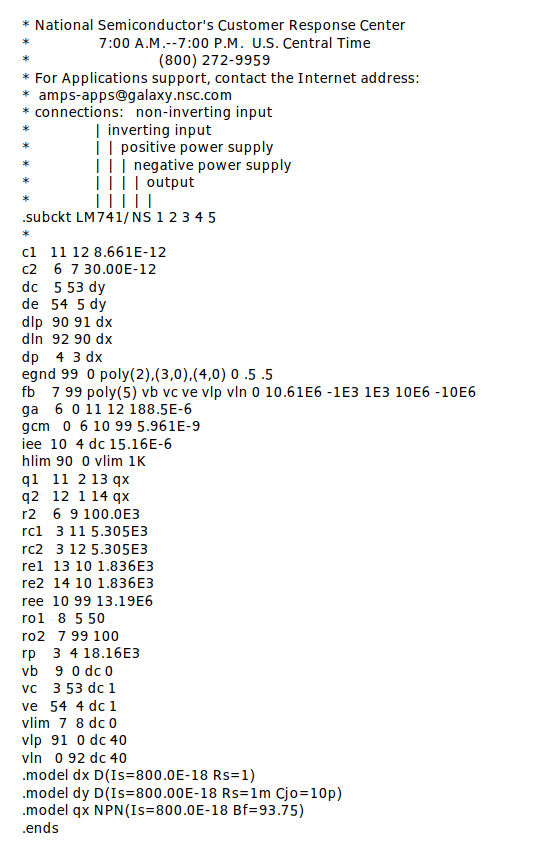
\includegraphics[width=0.8\linewidth]{figuras/oper1.png}
	\caption{Subcircuito que modeliza el LM741.}
	\label{oper1}
\end{figure}

Para comprender mejor este macromodelo se lo desarrolló en forma esquemática en la figura \ref{oper3}, allí se puede ver que los transistores $Q_1$ y $Q_2$ y sus resistencias asociadas emulan el amplificador diferencial de entrada, las fuentes de corriente controladas por tensión $g_a$ y $g_{cm}$ producen las ganancias de tensión de salida en modo diferencial y en modo común a través de la corriente que sensa la fuente $v_b$ que se transfiere a la salida a través de la fuente de corriente controlada por varias tensiones $B_1$ ($f_b$ en el macromodelo). En la fuente $B_1$ están incluidos los efectos de limitación de corriente de salida a través del sensado de las corrientes de las fuentes $v_{lim}$, $v_{lp}$ y $v_{ln}$ y de la saturación de la tensión de salida a través del sensado de las corrientes de las fuentes $v_b$ y $v_c$. Las capacidades $C_1$ y $C_2$ representan la respuesta en frecuencia y velocidad de respuesta del circuito.  


\begin{figure}
	\centering
	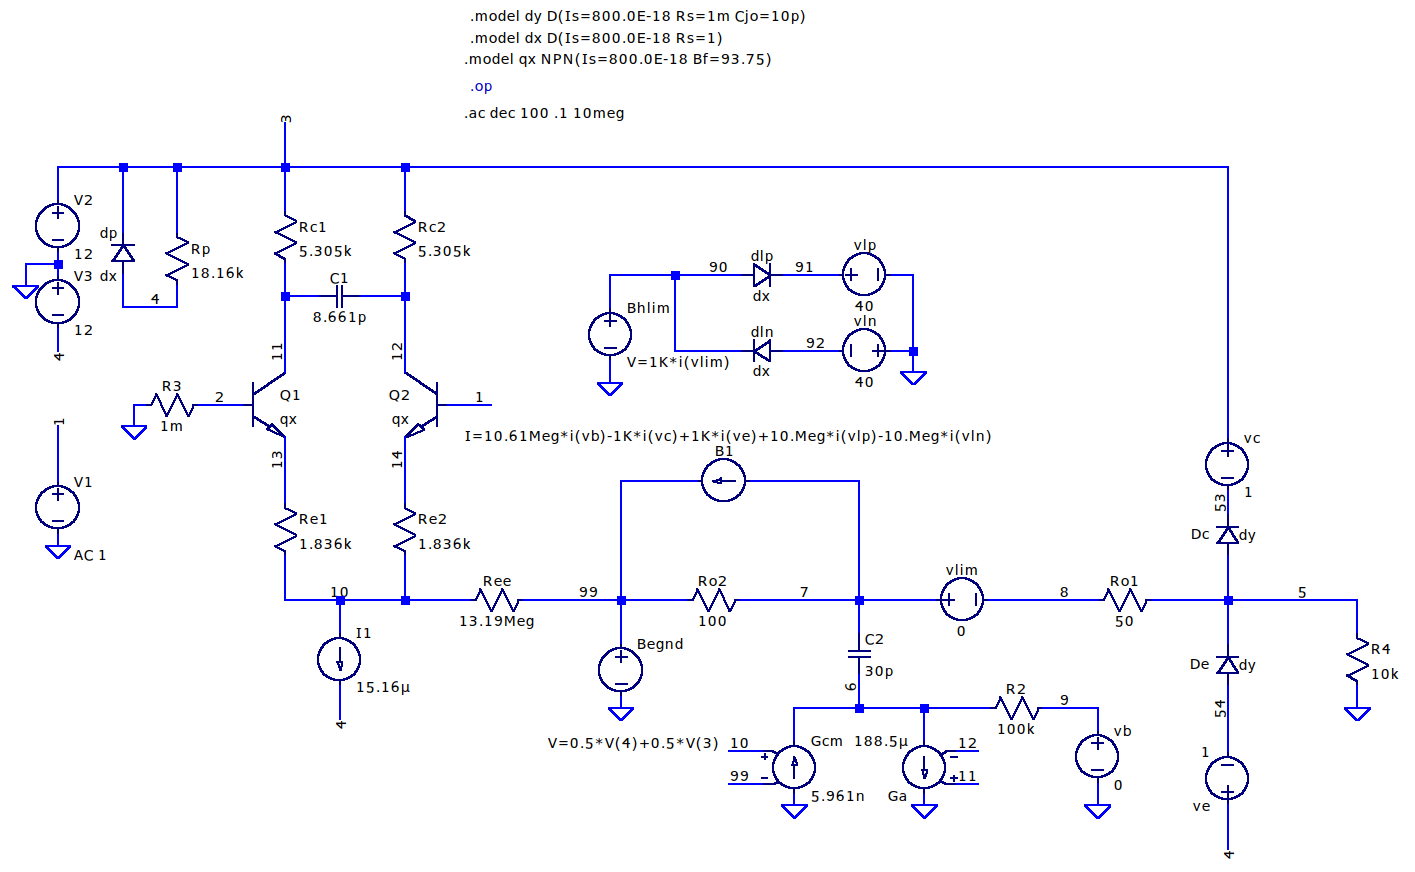
\includegraphics[width=0.9\linewidth]{figuras/oper3.png}
	\caption{Circuito esquemático que representa al macromodelo del LM741.}
	\label{oper3}
\end{figure}

Otra forma de modelizar un operacional sería utilizar el circuito a nivel componentes básicos como lo diseña el fabricante. Esto no es utilizado desde el punto de vista práctico, pero es útil para comprender el funcionamiento interno de los operacionales. En la figura \ref{oper2} se muestra un posible diseño simplificado. Los transistores $Q_1$ y $Q_2$ forman el par diferencial de entrada polarizados por la fuente $I_2$, los transistores $Q_3$ y $Q_4$ actúan como carga activa a la salida del par diferencial para proveer alta ganancia. $Q_5$ y $Q_6$ representan la etapa intermedia del amplificador proveyendo ganancia adicional. La etapa de salida clase AB está formada por los transistores $Q_7$ y $Q_8$, prepolarizados por los diodos $D_1$ y $D_2$ y la fuente $I_1$. El capacitor $C_1$  provee compensación por polo dominante. Se omitió la limitación de corriente por simplicidad.

\begin{figure}
	\centering
	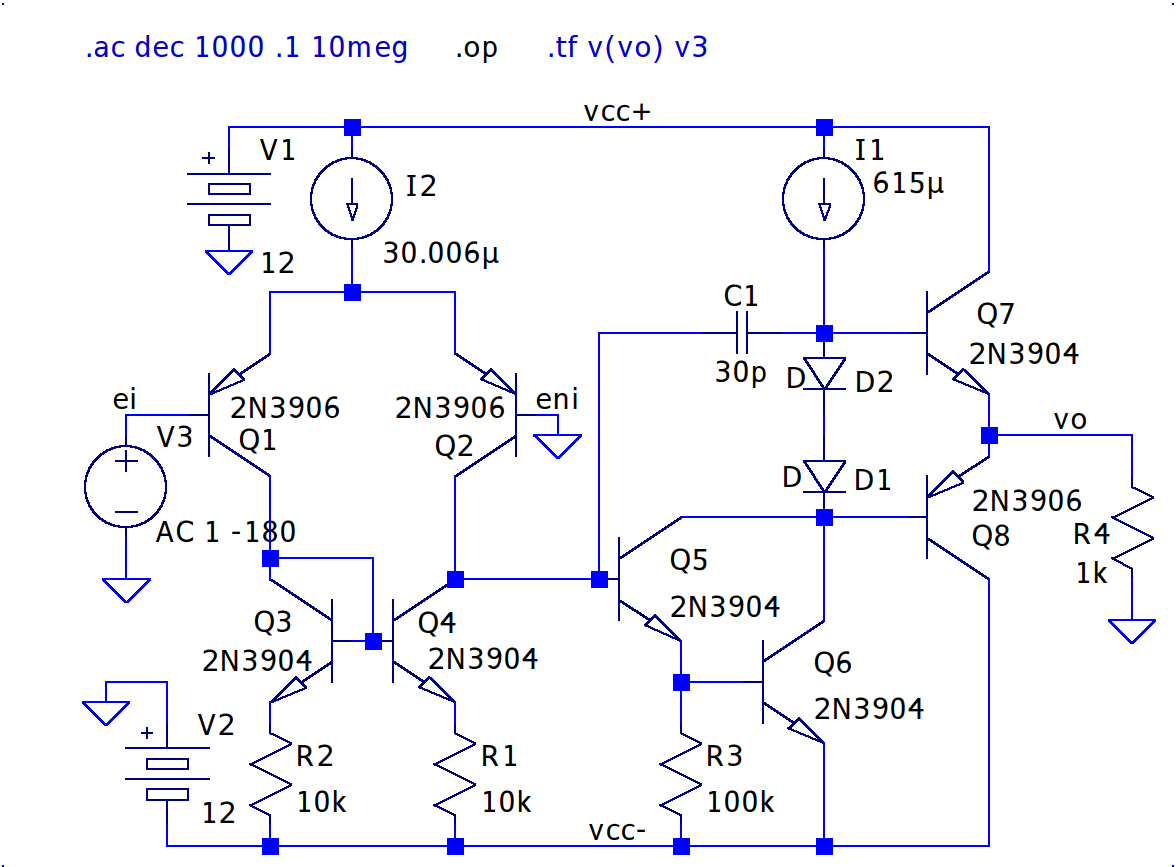
\includegraphics[width=0.8\linewidth]{figuras/oper2.png}
	\caption{Operacional genérico simplificado.}
	\label{oper2}
\end{figure}

Si al circuito de la figura \ref{oper2} se lo simula con la directiva \textit{.tf v(vo) v3}, que es la transferencia de continua entre salida y entrada, los resultados obtenidos son:

\bigskip


\begin{itemize}
	\item Ganancia $-1.29641e+06 \quad \quad (122.25dB)$
	\item Impedancia de entrada $996315 \Omega$
	\item Impedancia de salida $149.724 \Omega$
	
\end{itemize} 



Si  se lo simula con la directiva \textit{.ac dec 1000 .1 10meg}, que es el barrido de alterna, se pueden visualizar los diagrams de Bode de la ganancia de tensión cuyos resultados son:

\bigskip

\begin{itemize}
	\item Ganancia $122.24dB$, similar a lo obtenido por \textit{.tf}
	\item Frecuencia de corte (polo dominante) $2.18Hz$
	\item Margen de fase (para realimentación unitaria) $> 45\deg$
	
\end{itemize} 

El desajuste de continua en los amplificadores operacionales se modeliza utilizando los valores de tensión y corrientes proporcionados por los fabricantes en las hojas de datos. Estos son: tension de desajuste de entrada $V_{OS}$, corriente promedio de polarización de entrada $I_B$ y corriente de desajuste de entrada $I_{OS}$. En la figura \ref{oper4} se muestra como se aplica el modelo de desajuste típico, se anulan las fuentes externas, el operacional se considera ideal como una fuente de tensión controlada por tensión $E_1$ con una ganancia muy elevada, se le agrega en serie con la entrada una fuente de tensión $V_1$ que representa a $V_{OS}$ y se conectan respectivamente a las entradas $+$ y $-$ del operacional las fuentes de corriente $I_{B+}$ e $I_{B-}$ con el sentido correspondiente al tipo de amplificador diferencial de entrada que tenga el operacional. $I_{B+}$ e $I_{B-}$ pueden variar entre $I_{Bmax}=I_B+\frac{I_{OS}}{2}$ e $I_{Bmin}=I_B- \frac{I_{OS}}{2}$. 

Del circuito se ve que la expresión de la tensión de desajuste de la tensión de salida es:

\begin{equation}\label{ecuop1}
	V_o=\pm \big(1+\displaystyle \frac{R_1}{R_2} )V_{1}+R_1I_{B+}-R_3\big(1+\displaystyle \frac{R_1}{R_2} )I_{B-}
\end{equation}

El LM741 tiene los siguientes valores típicos de desajuste: $V_{OS}=1mV$, $I_B=80nA$ e $I_{OS}=20nA$. Maximizando y minimizando la ecuación \ref{ecuop1} queda $-7.545mV<V_o<7.545mV$. En este circuito el desajuste probable está centrado debido a que se diseña $R_3=R_1||R_2$ de modo de anular el efecto de la corriente de polarización promedio $I_B$.

Cuando el circuito es más complejo e involucra más operacionales, podría ser útil el método de simulación presentado en la figura \ref{oper4}, en el cual las fuentes de corriente $I_{B+}$ e $I_{B-}$  toman los valores aleatorios provenientes de la función del método de Monte Carlo \emph{mc(valor,tolerancia)} que usa un generador de números aleatorios para retornar un resultado entre $valor(1-tolerancia)$ y $valor(1+tolerancia)$. Similarmente la fuente $V_1$ toma el valor aleatorio de la función  \emph{flat(valor)}  dando un resultado entre $-valor$ y $+valor$ con distribución uniforme. La cantidad de combinaciones realizadas se dimensiona con el barrido del parámetro $n$ utilizando la directiva \emph{.step param n 0 999 1}, en este caso se obtienen 1000 combinaciones aleatorias de las fuentes $I_{B+}$, $I_{B-}$ y $V_1$. En la figura \ref{oper5} se muestra el valor de la salida $V_o$ para cada una de las 1000 combinaciones aleatorias ensayadas, notándose que los valores máximos y mínimos obtenidos coinciden aproximadamente con los obtenidos por cálculo brindando una estimación satisfactoria.  


\begin{figure}
	\centering
	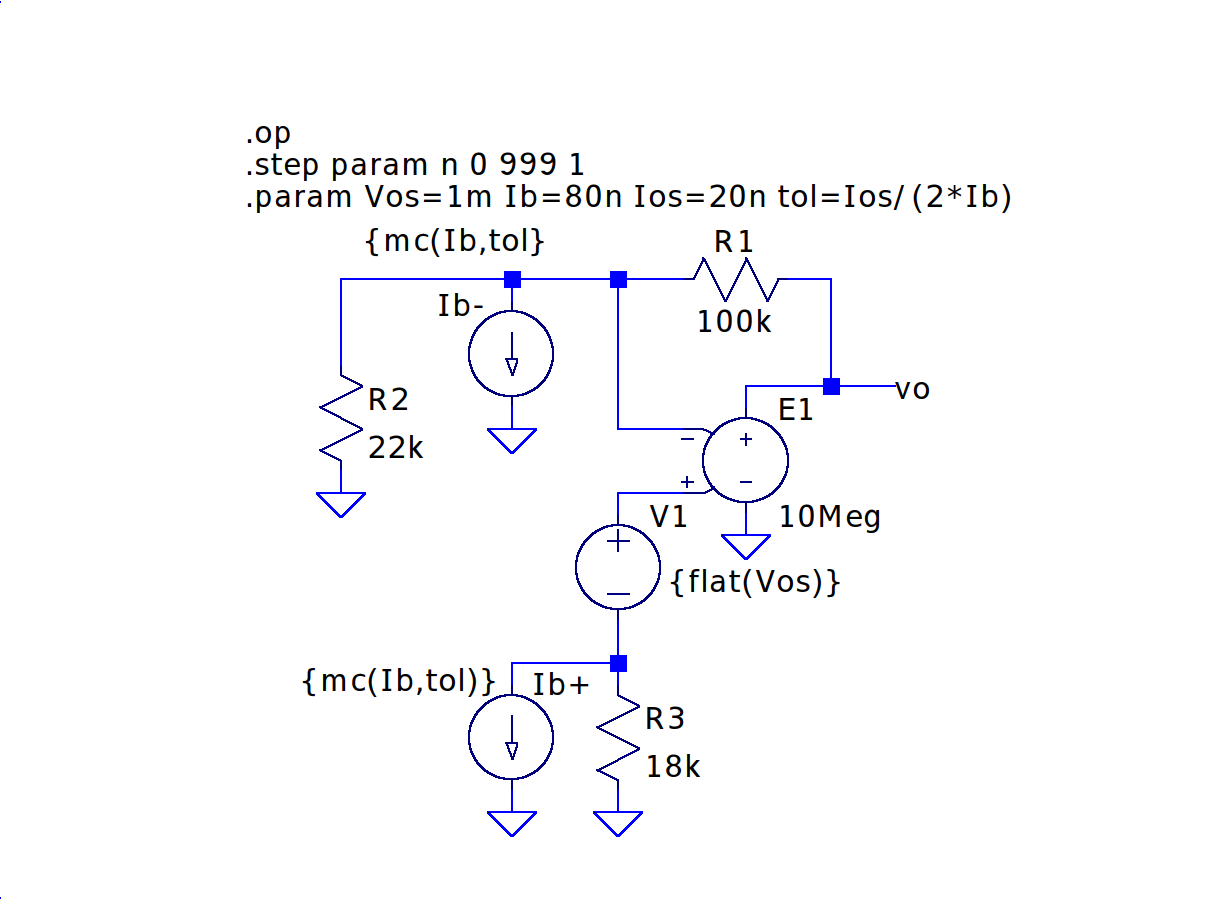
\includegraphics[width=0.8\linewidth]{figuras/oper4.png}
	\caption{Modelo de desajuste de un Operacional.}
	\label{oper4}
\end{figure}

\begin{figure}
	\centering
	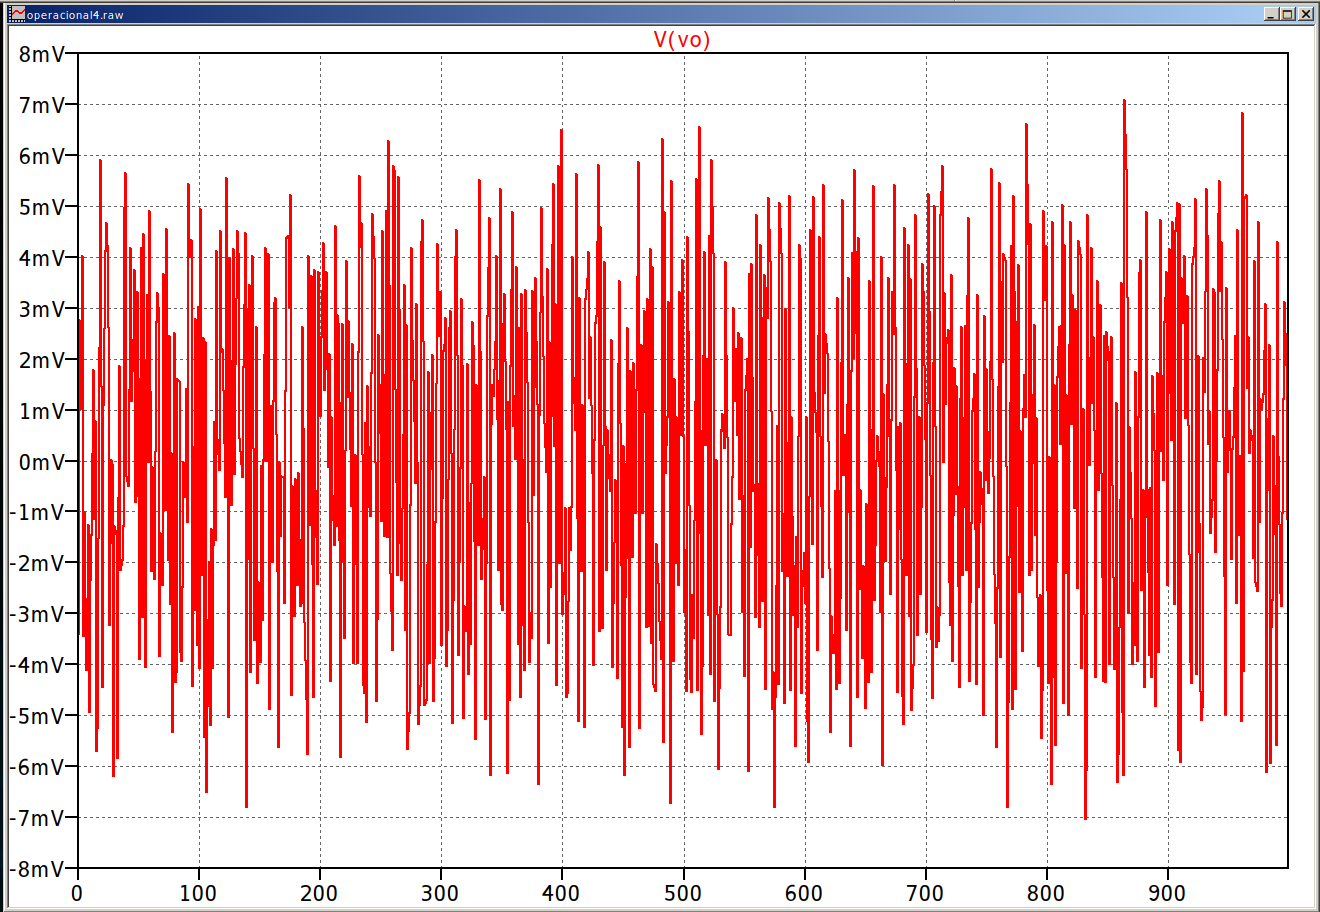
\includegraphics[width=0.8\linewidth]{figuras/oper5.png}
	\caption{Estimación del desajuste con las funciones de Monte Carlo y Flat.}
	\label{oper5}
\end{figure}


La respuesta temporal de los modelos de los operacionales se pueden evaluar utilizando la directiva \emph{.tran}. Los circuitos de la figura \ref{oper6} representan el ensayo de la respuesta a un pulso de $5\mu s$ de un circuito seguidor implementado con un $LM741$, en el circuito de la izquierda el pulso es de $1V$ de amplitud y en el de la derecha de $100mV$. 

En la figura \ref{oper7} se muestran los resultados de la simulación. En la parte superior se grafican el pulso de entrada de $100mV$ de amplitud y $5\mu s$ de duración y la salida correspondiente, se puede observar que en este caso el operacional está actuando en función de la respuesta en frecuencia de su transferencia lineal. En el caso de la parte inferior de la figura (amplitud de $1V$), se observa que está actuando la limitación no lineal de la máxima velocidad de subida y bajada del operacional, se puede estimar esa velocidad observando que le toma aproximadamente $2\mu s$ subir de $0$ a $1V$, es decir que sube (y baja) a $\approx 0.5V/\mu s$, que es el valor del \emph{slew rate} porporcionado por la hoja de datos del $LM741$.


\begin{figure}
	\centering
	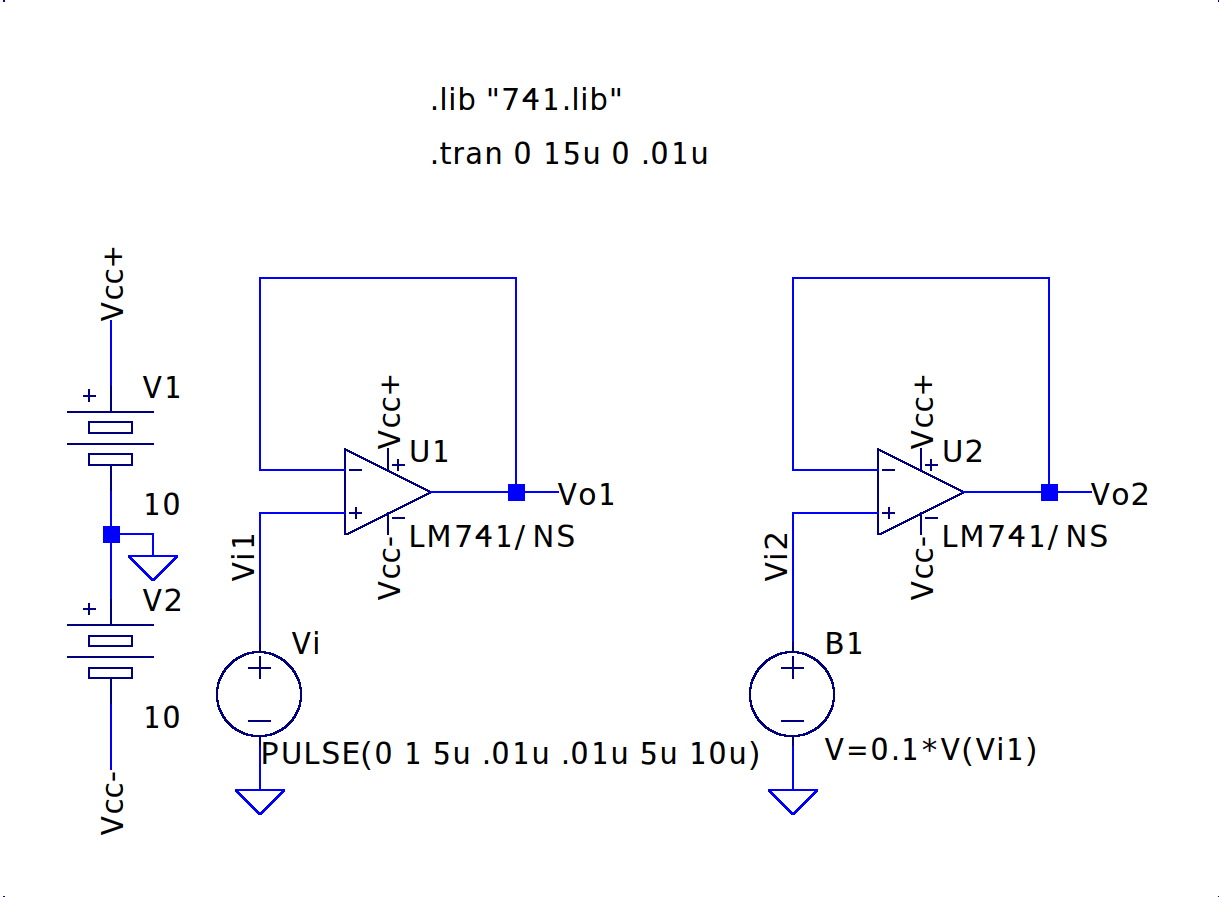
\includegraphics[width=0.8\linewidth]{figuras/oper6.png}
	\caption{Circuito seguidor con Operacional.}
	\label{oper6}
\end{figure}

\begin{figure}
	\centering
	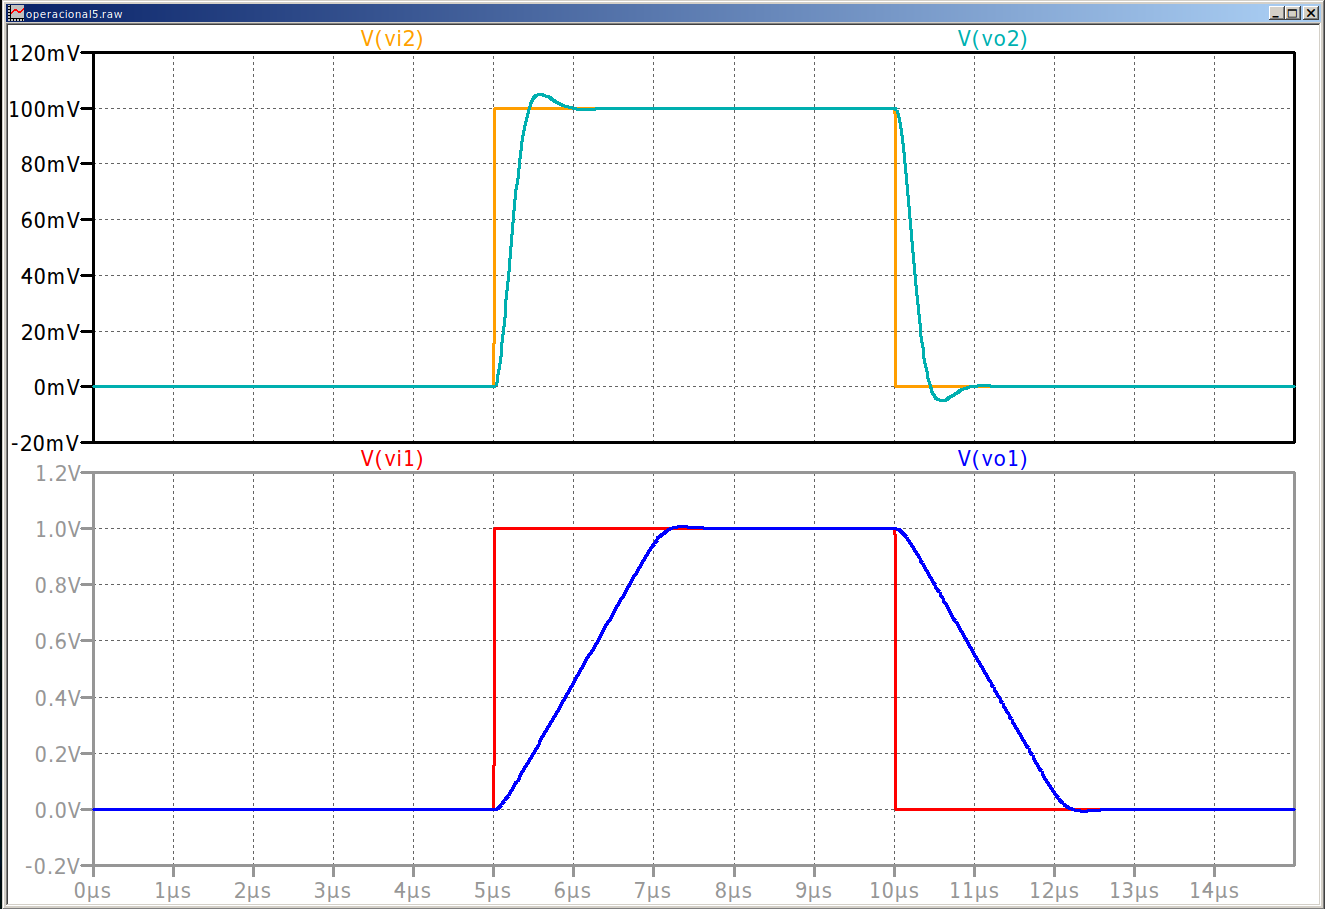
\includegraphics[width=0.8\linewidth]{figuras/oper7.png}
	\caption{Respuesta a pulsos del seguidor.}
	\label{oper7}
\end{figure}


La relación de rechazo al modo común CMRR es una característica importante a tener en cuenta en los amplificadores diferenciales en general y por lo tanto también en los operacionales. Cuantifica el cociente entre la ganancia en modo diferencial y la ganancia en modo común medido en $dB$. Cuanto más grande sea, más eficiente será el rechazo a las señales de modo común, por lo general señales no deseadas en un amplificador diferencial.

En la figura \ref{oper8} se muestra un amplificador diferencial simple implementado con un LM741. Las entradas diferenciales son las fuentes $V_{d1}$ y $V_{d2}$, la fuente $V_{mc}$ simula la señal de modo común. Cuando las 4 resistencias son iguales la ganancia diferencial es $V_o/(V_{d2}-V_{d1})=1$. Por otro lado en este mismo caso la ganancia de modo común $\rightarrow \infty$ si el operacional es ideal y aproximadamente igual al CMRR del operacional si éste es real debido a que la ganancia diferencial es 1. La CMRR del LM741, según su hoja de datos, es de $90dB$.

La CMRR se ve muy afectada, a la baja, cuando las resistencias no son exactamente iguales, por lo que las tolerancias de las resistencias utilizadas deben ser muy tenidas en cuenta. En el circuito de la figura \ref{oper8} se simula por método de Monte Carlo el circuito utilizando resistencias al $1\%$. 

En primera instancia se simuló la ganancia diferencial $A_d$ utilizando la directiva \emph{.tran}, como la fuente de modo común es de AC la simulación temporal la considera nula. La ganancia diferencial se mantuvo entre $0.983<A_d<1.015$ en los 100 casos estadísticos simulados teniendo en cuenta la tolerancia del $1\%$ en las resistencias, muy similar al valor teórico.

Luego se simuló la ganancia de modo común $A_{mc}$ utilizando la directiva \emph{.ac}, en este barrido de alterna las fuentes $V_{d1}$ y $V_{d2}$ son consideradas nulas. En la figura \ref{oper9} se muestran las 100 simulaciones obtenidas con las combinaciones aleatorias de las resistencias con su tolerancia. Como se puede suponer que la ganancia diferencial es igua1 a 1 y la fuente de entrada de modo común es de $1V$, el eje vertical de la figura puede interpretarse como la CMMR cambiada de signo, es decir que la CMRR puede bajar aproximadamente hasta al menos $35dB$ en las combinaciones aleatorias simuladas.  
 


\begin{figure}
	\centering
	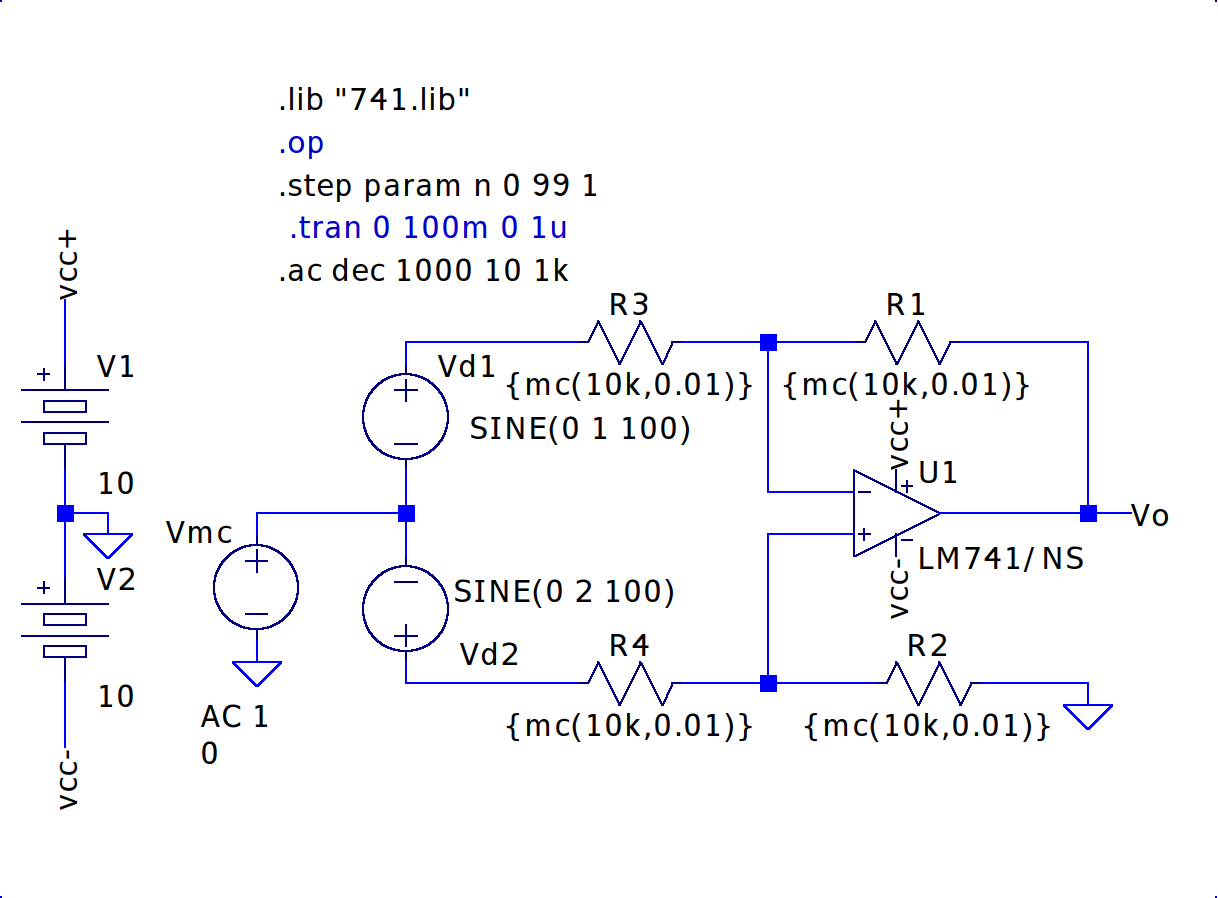
\includegraphics[width=0.8\linewidth]{figuras/oper8.png}
	\caption{Amplificador diferencial.}
	\label{oper8}
\end{figure}

\begin{figure}
	\centering
	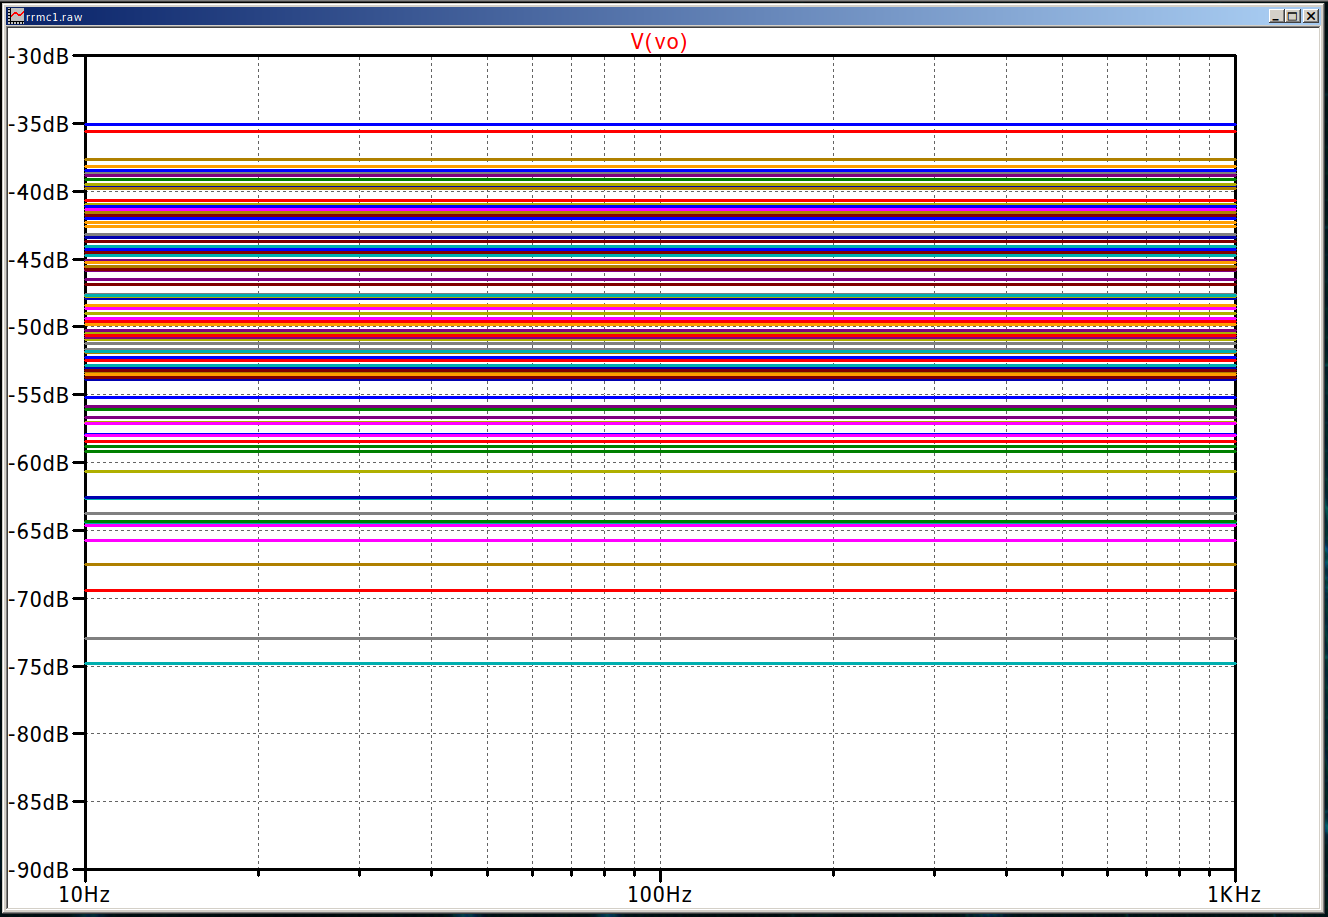
\includegraphics[width=0.8\linewidth]{figuras/oper9.png}
	\caption{CMRR teniendo en cuenta las tolerancias de las resistencias.}
	\label{oper9}
\end{figure}

\section{Aplicaciones con Operacionales }
%
\hspace{10pt} En esta sección se presentan algunos ejemplos de simulaciones de circuitos que utilizan Amplificadores Operacionales.

El circuito dibujado a la izquierda en la figura \ref{oper10} representa un integrador donde idealmente la salida debería ser:



\begin{equation}\label{ecuop2}
	 V{o1}(t)=\displaystyle -\frac{1}{R_1C_1}\int_{o}^{t}V_i(t)dt+V_{o1}(0)
\end{equation}





El gáfico superior de la figura \ref{oper11} muestra la respuesta temporal del circuito mencionado anteriormente cuando la entrada es una onda cuadrada de $500Hz$ con amplitud de $\pm 1V$. Si bien la forma de onda de la salida se corresponde con la respuesta esperada por el integrador, se ve que el caracter no ideal del operacional con respecto a las corrientes de desajuste de entrada llevan a que el extremo superior de la respuesta esté anclado en la saturación de la fuente $V_{cc+}$. Para evitar este inconveniente  en el circuito de la derecha de la figura \ref{oper10} se coloca en paralelo con el capacitor una resistencia que le da camino a la corriente de desajuste de continua y evita la carga constante del capacitor, esta resistencia debe ser lo suficientemente grande para que a la frecuencia de trabajo del integrador no influya apreciablemente en su respuesta. En el gráfico inferior de la figura \ref{oper11} se ve que la respuesta es similar al caso anterior, pero centrada en el entorno de $\approx 0V$.



\begin{figure}
	\centering
	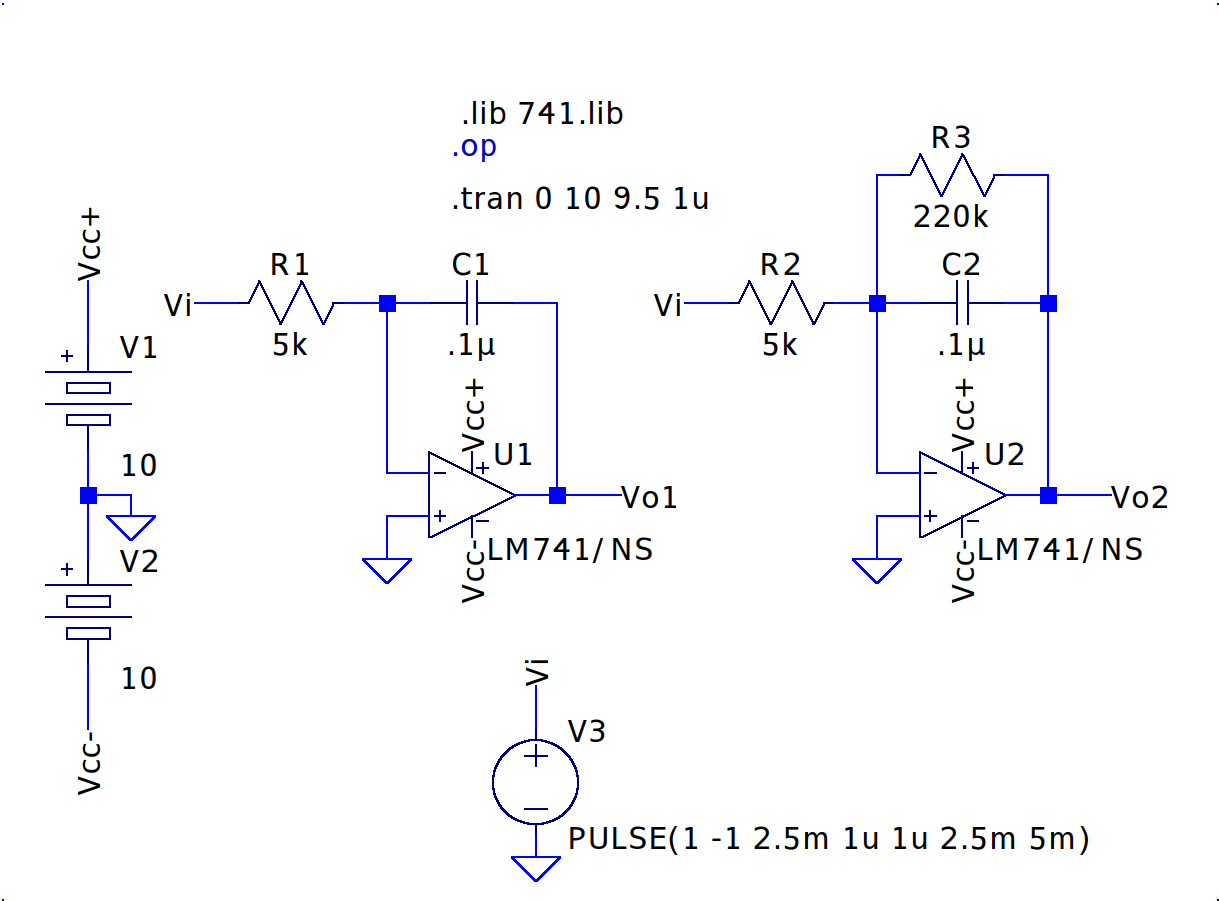
\includegraphics[width=0.8\linewidth]{figuras/oper10.png}
	\caption{Integrador con Operacional.}
	\label{oper10}
\end{figure}

\begin{figure}
	\centering
	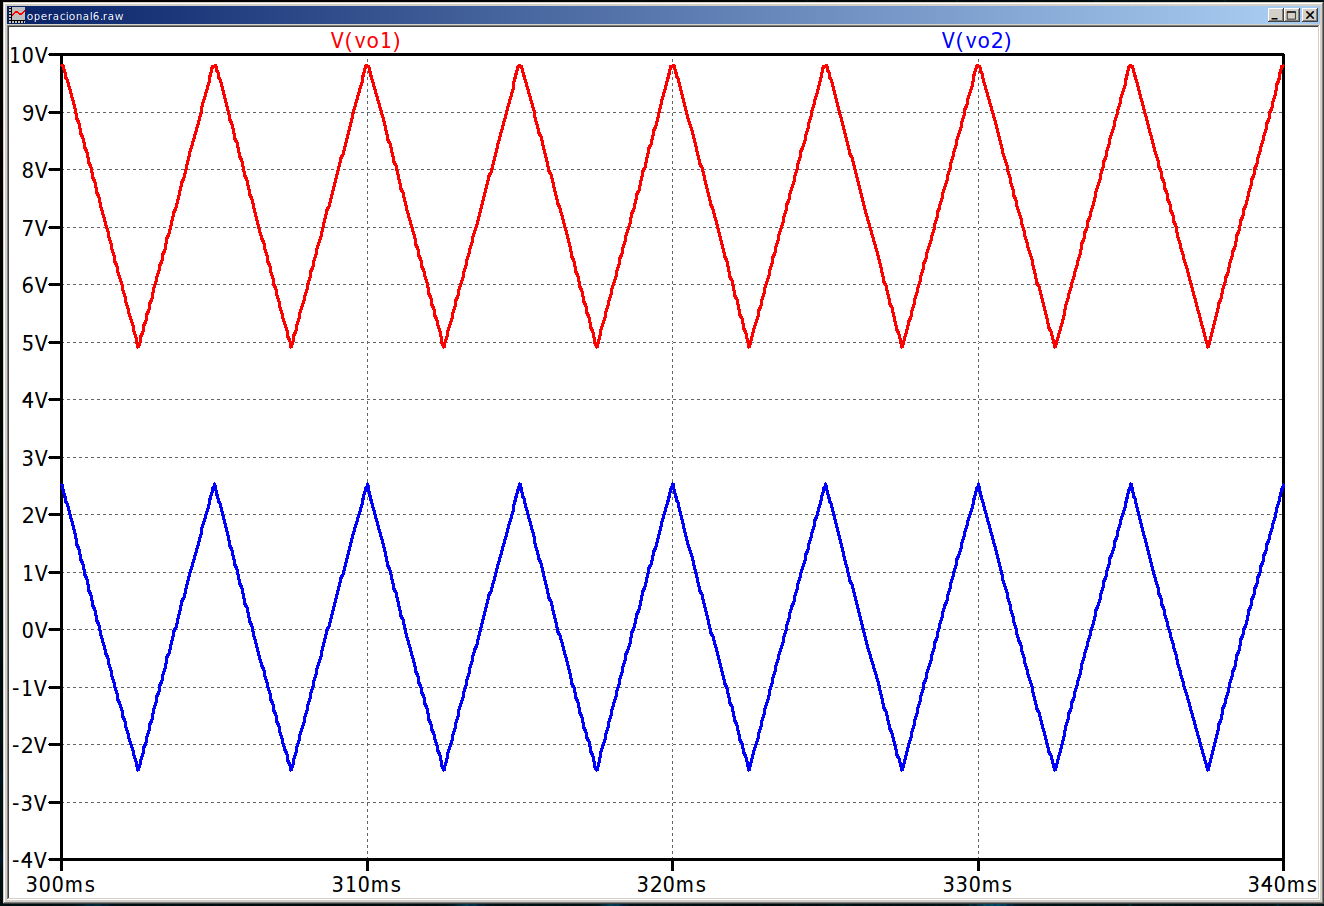
\includegraphics[width=0.8\linewidth]{figuras/oper11.png}
	\caption{Respuesta temporal del integrador a una onda cuadrada.}
	\label{oper11}
\end{figure}


El circuito de la figura \ref{oper12}  es un derivador ideal si se considera $R_2=0$ y se anula la fuente auxiliar $V_4$, respondiendo a la expresión:

 \begin{equation}\label{ecuop3}
 	V{o1}(t)=\displaystyle -R_1C_1\frac{dV_3}{dt}
 \end{equation}
 
 Este derivador ideal tiene el inconveniente de tender a ser inestable o con un margen de fase exiguo, y como la ganancia de tensión aumenta a medida que aumenta la frecuencia lo hace muy ruidoso. Para solucionar estos inconvenientes se le agrega en serie con el capacitor la resistencia $R_2$ que lo tiende a compensar y le da un límite a la ganancia a altas frecuencias. En la figura \ref{oper13} se muestra la simulación temporal de la salida si la entrada es una onda cuadrada, para los valores de $R_2\approx0$ y $R_2=100\Omega$, en ella se ve la tendencia a oscilar en el primer caso y la respuesta típica de un derivador real en el segundo.
 
 En la figura \ref{oper14} se muestra la simulación de la ganancia de lazo (ver capìtulo 3) utilizando la fuente auxiliar $V_4$ y anulando la entrada, para los dos casos de $R_2$ ya presentados. En ella se ve que para $R_2\approx0$ el margen de fase es casi nulo y para $R_2=100\Omega$ aumenta considerablemente.
 
 
 \begin{figure}
 	\centering
 	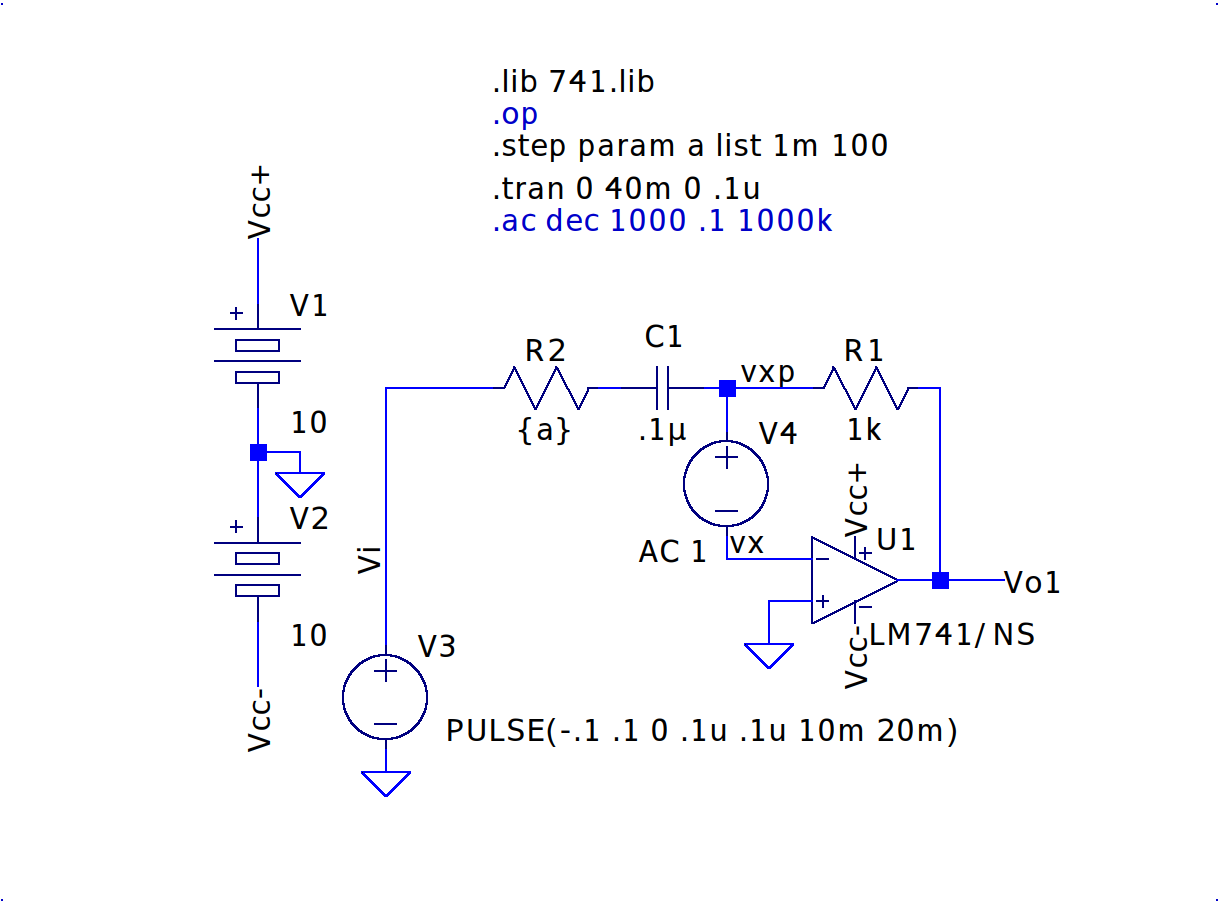
\includegraphics[width=0.8\linewidth]{figuras/oper12.png}
 	\caption{Derivador con Operacional.}
 	\label{oper12}
 \end{figure}
 
 
 \begin{figure}
 	\centering
 	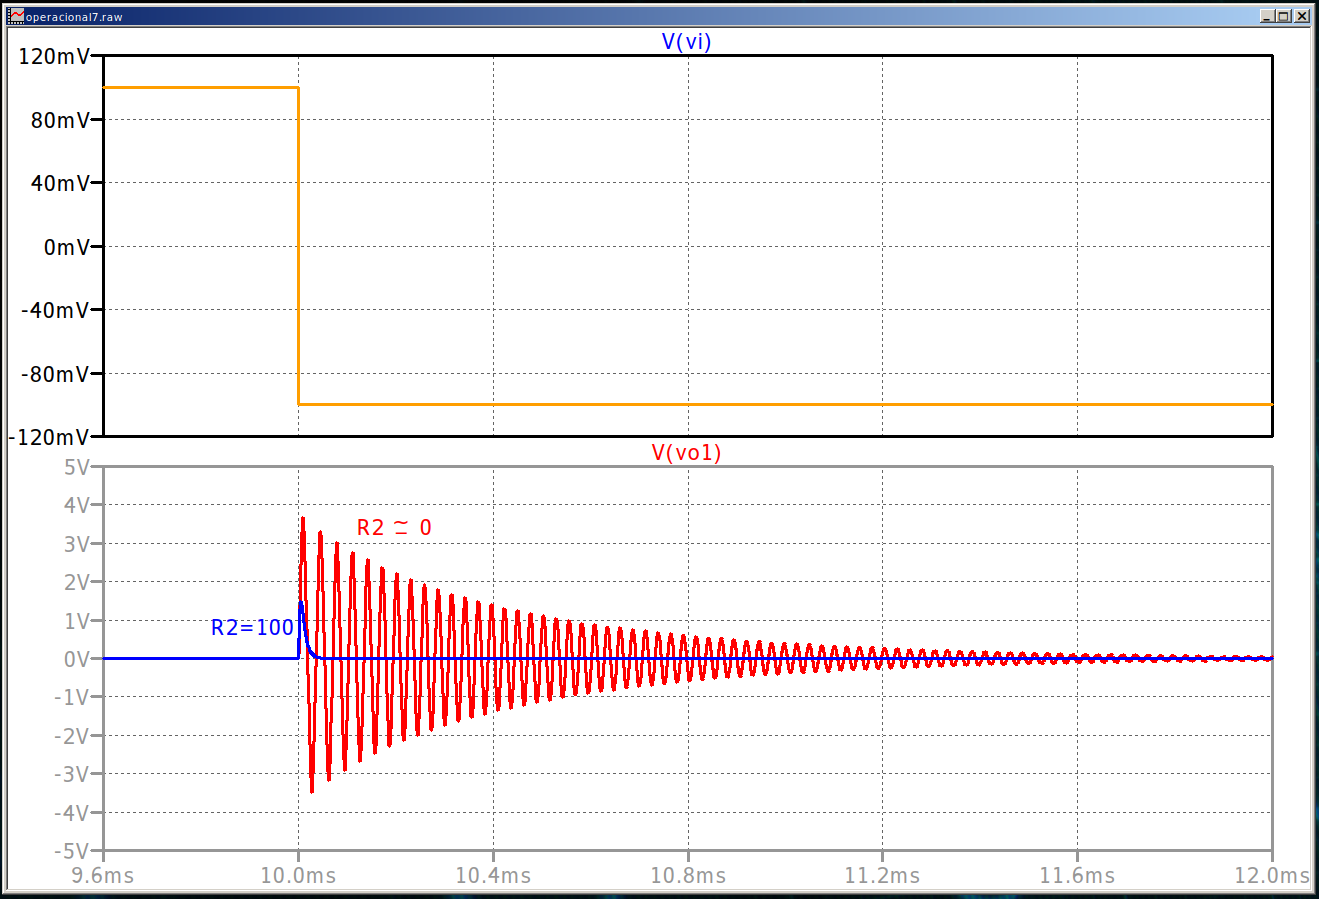
\includegraphics[width=0.8\linewidth]{figuras/oper13.png}
 	\caption{Respuesta temporal del derivador a una onda cuadrada.}
 	\label{oper13}
 \end{figure}
 
 \begin{figure}
 	\centering
 	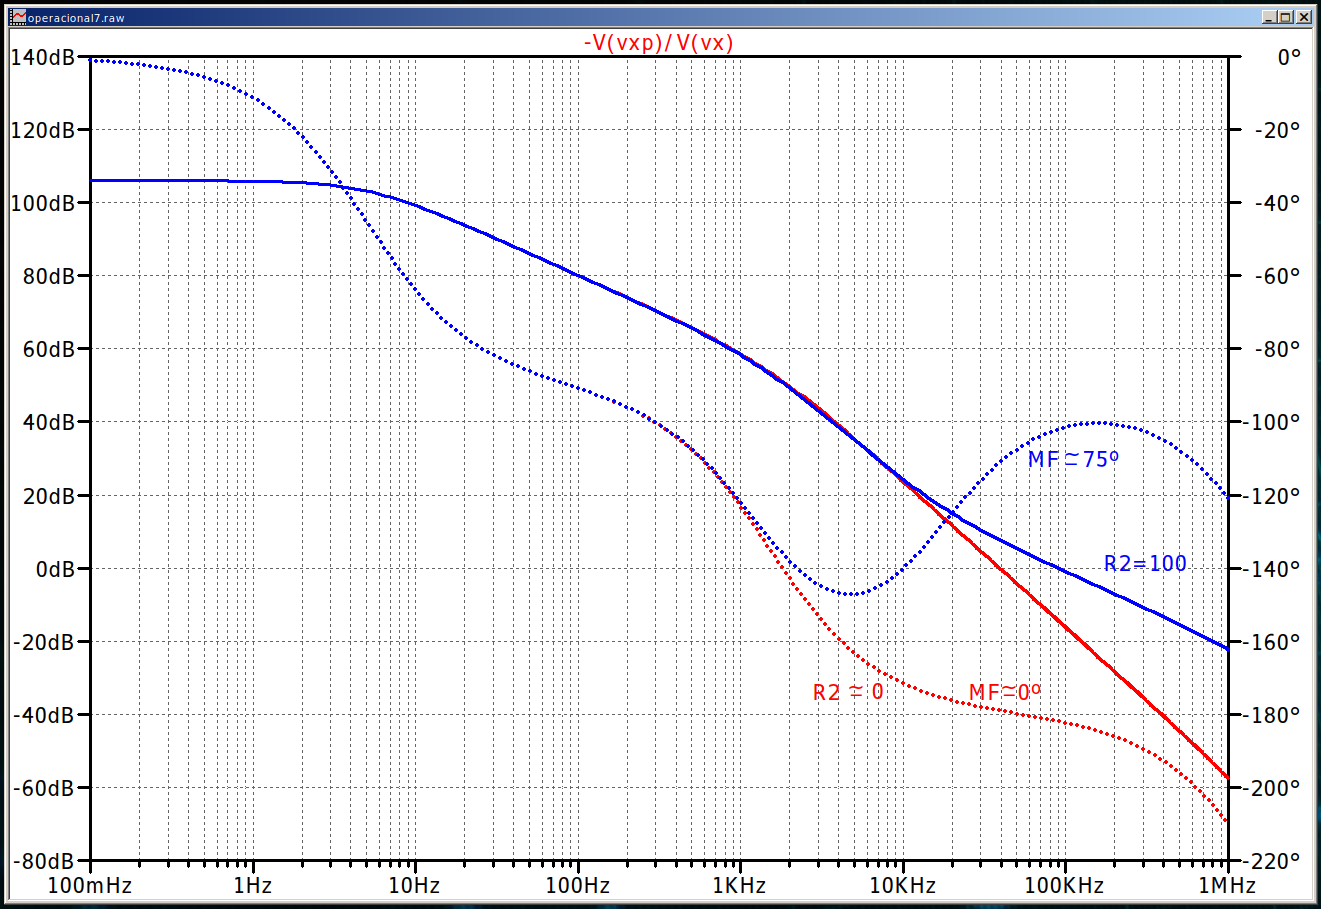
\includegraphics[width=0.8\linewidth]{figuras/oper14.png}
 	\caption{Ganancia de lazo del derivador.}
 	\label{oper14}
 \end{figure}
 
 Los Amplificadores Operacionales son utilizados ampliamente para implementar filtros activos. Un ejemplo es el filtro pasa banda de segundo orden mostrado en la figura \ref{oper15}, la transferencia de dicho filtro es:
 
  
 \begin{equation}\label{ecuop4}
 	\displaystyle \frac{V_o}{V_i}(S)= \displaystyle \frac{1}{S^2C_1C_2R_1R_2+SC_2(R_1+R_2)+1}
 \end{equation}
 
 
 La frecuencia central, el factor de calidad y el ancho de banda  teóricos son:
 
 \begin{equation}\label{ecuop5}
 f_o= \displaystyle \frac{1}{2 \pi \sqrt{C_1C_2R_1R_2}}=1.56KHz \quad Q=\displaystyle \frac{1}{2\pi f_oC_2(R_1+R_2)}=10.85 \quad B_f=\displaystyle \frac{f_o}{Q}=143.8Hz \quad A_o=20.70dB
 \end{equation}
 
 En la figura \ref{oper16} se muestra la simulación de la transferencia en el dominio de la frecuencia utilizando la directiva \emph{.ac lin 10000 1k 2k }, en ella se ve que los datos simulados ($f_o=1.53KHz \quad B_f=140.5HZ \quad A_o=20.77dB$ ) coinciden aproximadamente con los teóricos.
 
 
   \begin{figure}
  	\centering
  	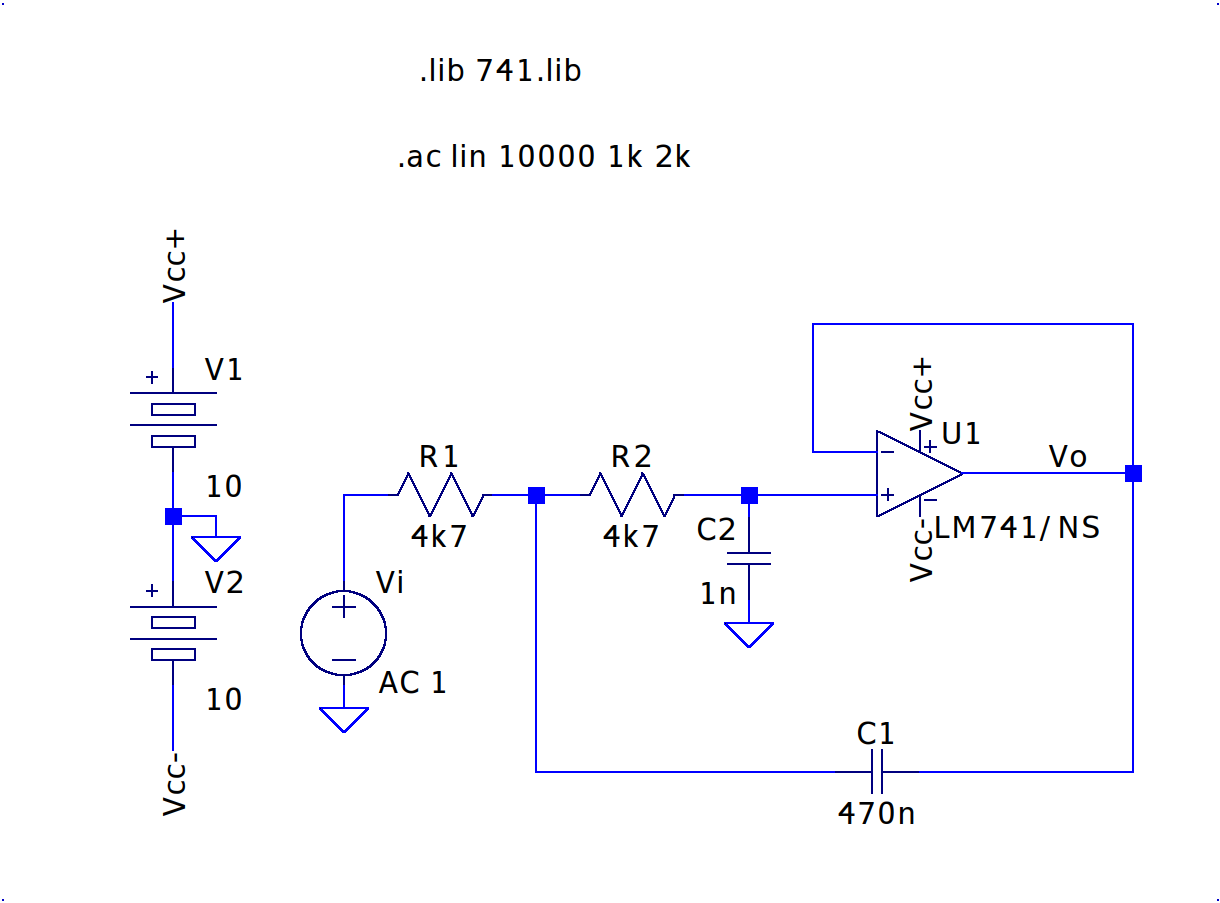
\includegraphics[width=0.8\linewidth]{figuras/oper15.png}
  	\caption{Filtro activo pasa banda de segundo orden.}
  	\label{oper15}
  \end{figure}
  
  \begin{figure}
  	\centering
  	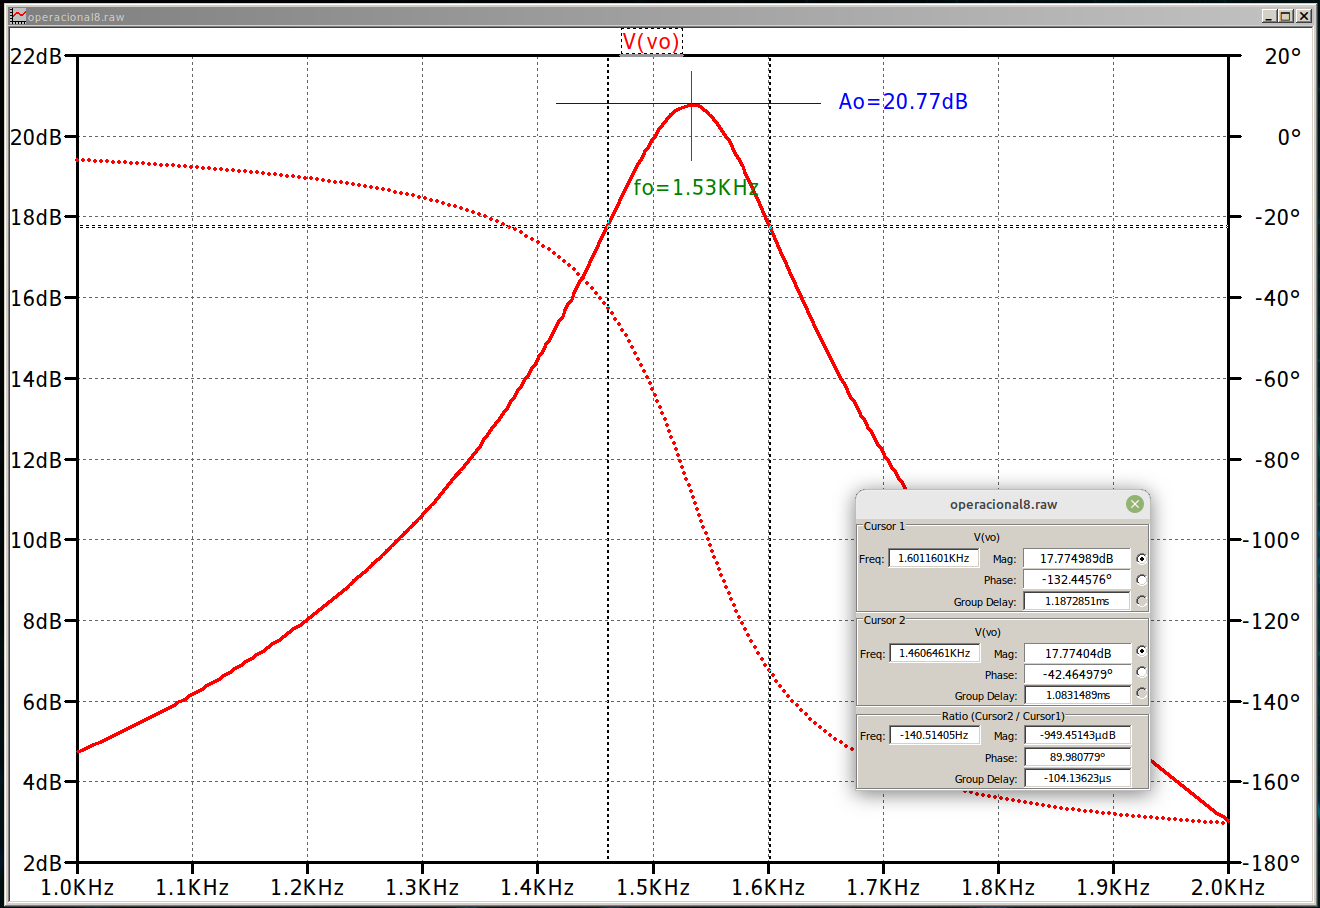
\includegraphics[width=0.8\linewidth]{figuras/oper16.png}
  	\caption{Respuesta en frecuencia del circuito de la figura \ref{oper15}.}
  	\label{oper16}
  \end{figure}
  
  
  Otras aplicaciones de AC utilizando operacionales son circuitos modificadores de impedancia tales como giradores de impedancia y multiplicadores capacitvos. Un ejemplo es el circuito de la figura \ref{oper17}, que presenta a la entrada una impedancia con características inductivas sin la utilización de inductores físicos. La impedancia de entrada teórica está dada por:
  
  \begin{equation}\label{ecuop6}
  	Z_i= R_2+jwC_1R_1R_2
  \end{equation}
  
  Si la entrada es una señal senoidal de frecuencia $1KHz$ la impedancia de entrada sería  teóricamente $Z_i=100\Omega + j 638.32\Omega$. En la figura \ref{oper18} se muestra la simulación del circuito utilizando la directiva \emph{.ac dec 10000 1 10K} graficando la impedancia de entrada en función de la frecuencia entre $1Hz$ y $10KHz$, esto se logra con la visualización de la magnitud $V(v_i)/-I(V_3)$, el signo negativo de la corriente $I(V_3)$ se debe a que en LTSpice  las corrientes sobre las fuentes de tensión se consideran positivas cuando circulan del polo positivo hacia el negativo de la fuente. Con el cursor posicionado en $f=1KHz$ los resultado son $|Z_i|=56.183dB\Omega \quad (644.36\Omega)$ y $\phi_{Z_i}=80.96^{\circ} $, es decir $Z_i=101.27\Omega + j 636.36\Omega$ que son valores similares a los teóricos. A mayores frecuencias comienzan a verse los efectos de la capacidad de entrada y de la respuesta en frecuencia de los operacionales reales lo que lo aleja del comportamiento teórico.
  
  Puede simularse también la respuesta temporal del circuito de la figura \ref{oper17} con la directiva \emph{.tran 0 100m 90m 0.05u}, en este caso se utiliza una fuente senoidal de entrada de $\pm1V$ de ampiltud y de $f=1KHz$. Los resultados se ven el la figura \ref{oper19}, en la parte inferior se muestran la tensión de entrada $V(v_i)$ y la corriente de entrada $-I(V_3)$ en función del tiempo, si se realiza el cociente de los fasores que representan esas dos magnitudes se obtienen valores similares de los de $Z_i$ obtenidos del gráfico de la figura \ref{oper18}. En la parte superior se representa la salida del operacional $V_o$, dando valores dentro del rango de funcionamiento del mismo.
  
  \begin{figure}
  	\centering
  	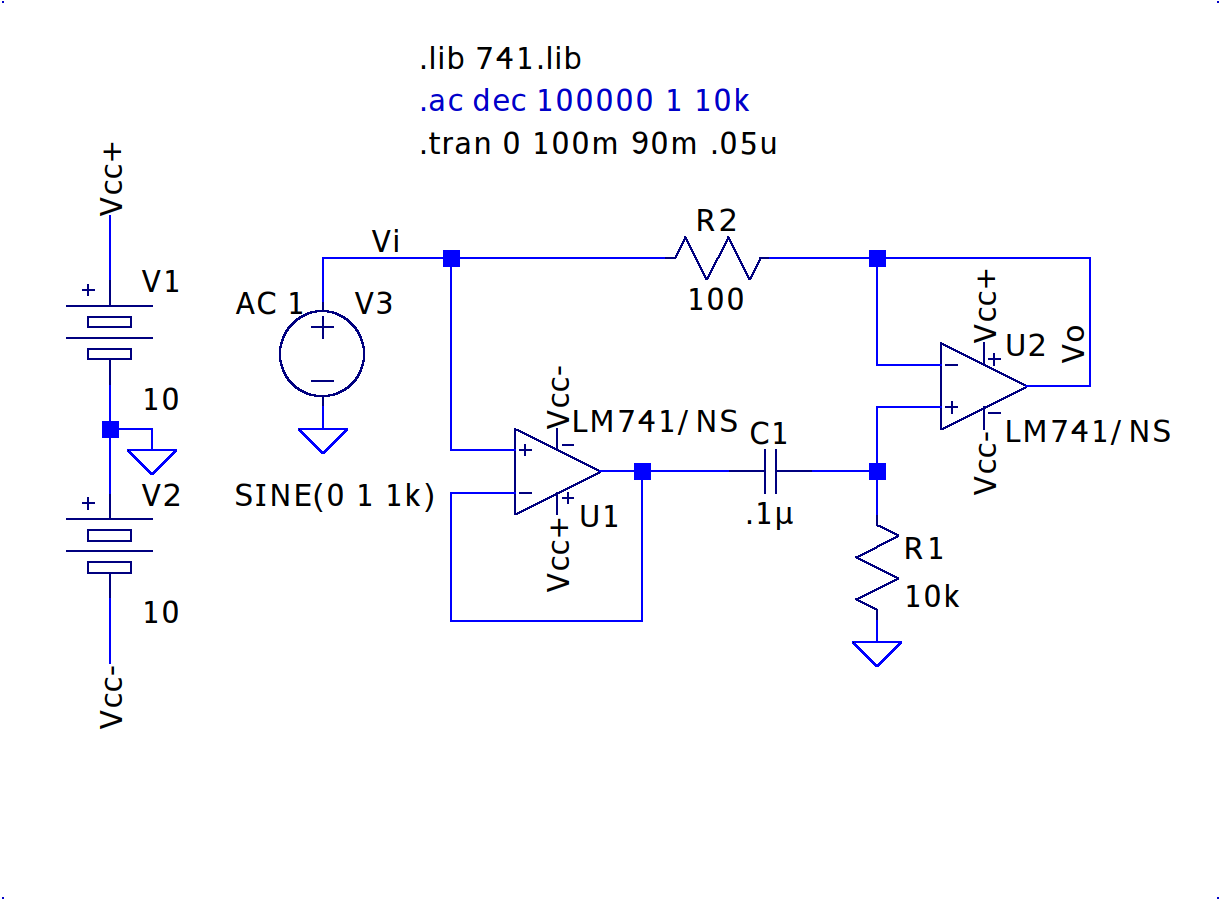
\includegraphics[width=0.8\linewidth]{figuras/oper17.png}
  	\caption{Girador de impedancia.}
  	\label{oper17}
  \end{figure}
  
  \begin{figure}
  	\centering
  	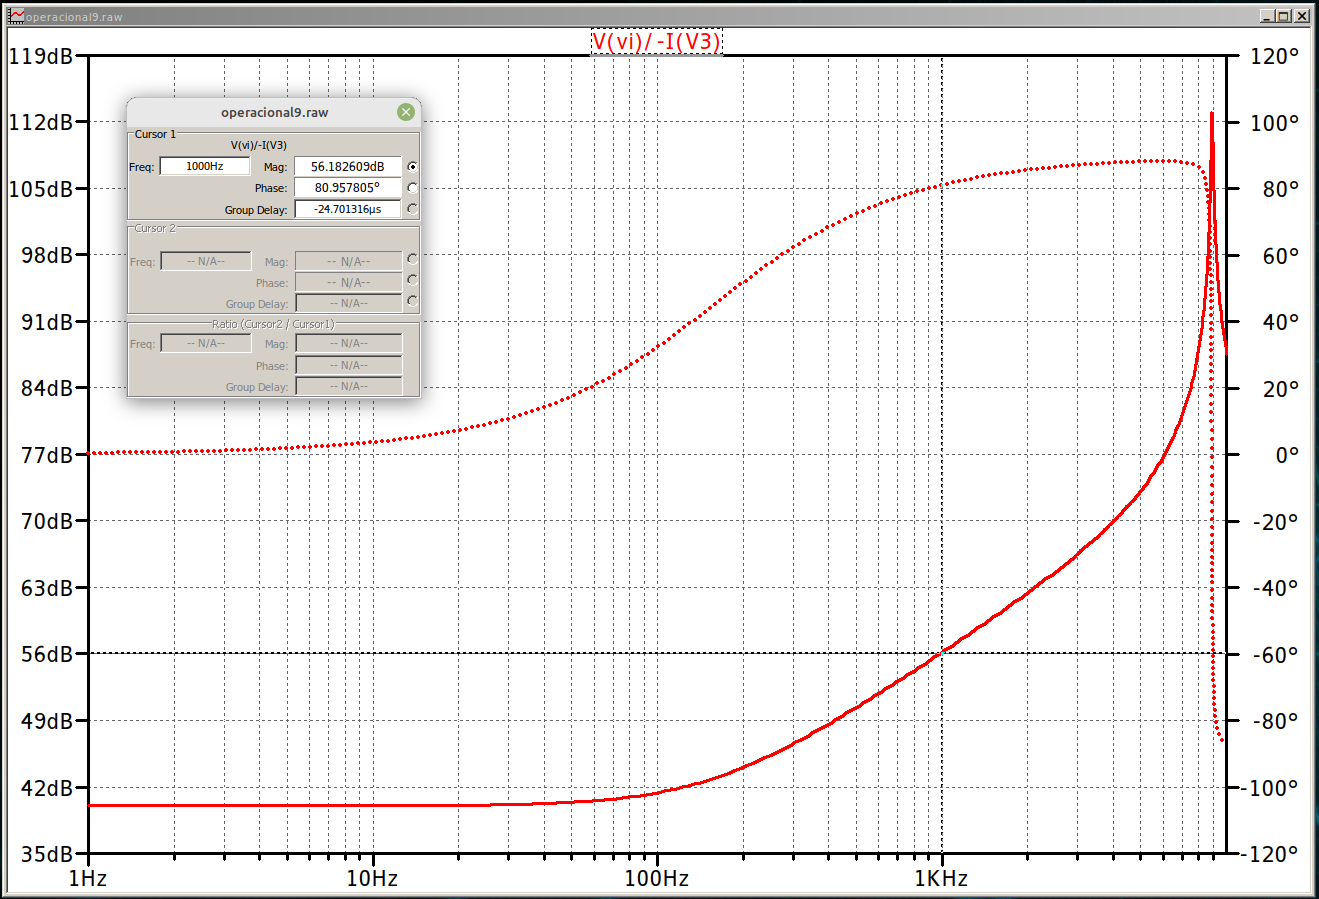
\includegraphics[width=0.8\linewidth]{figuras/oper18.png}
  	\caption{Impedancia de entrada en función de la frecuencia del circuito de la figura \ref{oper17}.}
  	\label{oper18}
  \end{figure}
  
  
  \begin{figure}
  	\centering
  	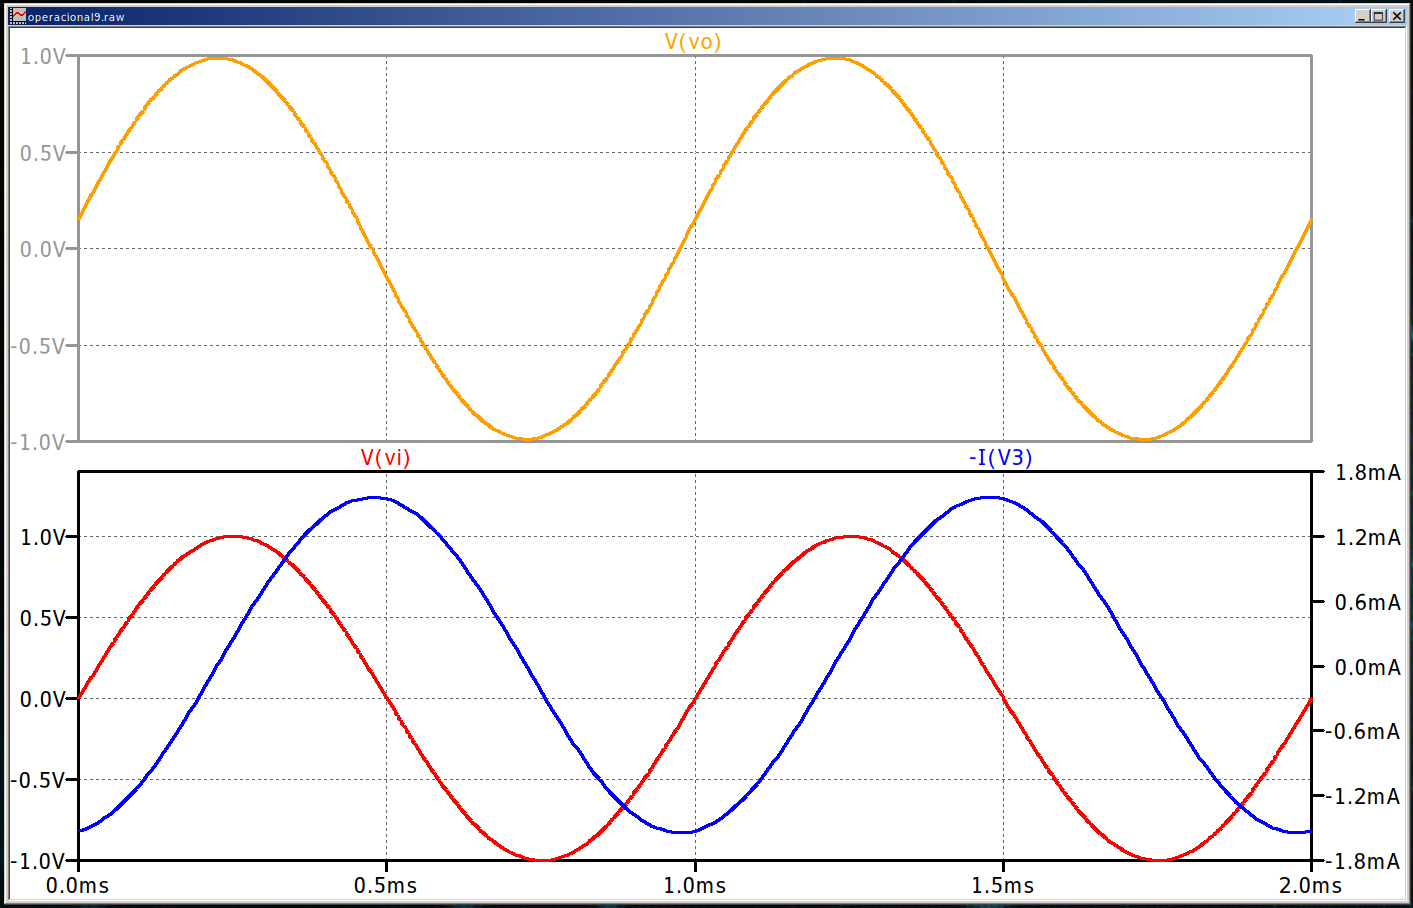
\includegraphics[width=0.8\linewidth]{figuras/oper19.png}
  	\caption{Respuesta temporal del circuito de la figura \ref{oper17}.}
  	\label{oper19}
  \end{figure}
  
  El circuito de la figura \ref{oper20} es un ejemplo de aplicaciones no lineales de Operacionales en conjunción con diodos. Haciendo el análisis teórico se demuestra que para $C_1=0$ y con $R_4$ ajustada para que sea $\approx \pi  \times 10K\Omega$ la transferencia sería:
  
  \begin{equation}\label{ecuop7}
  \begin{split}
  Si \quad V_3\geq 0, \qquad \frac{V_o}{V_3}&=  \left(\frac{R_4R_2}{R_7R_1}-\frac{R_4}{R_5}\right) \approx \frac{\pi}{2} \\
  Si \quad V_3<0, \qquad \frac{V_o}{V_3}&= \left(-\frac{R_4}{R_5}\right) \approx -\frac{\pi}{2}
  \end{split} 
  \end{equation}
  	
  La simulación de la  transferencia bajo estas condiciones está dada por la directiva \emph{.dc v3 -5 5 1m}, que es el barrido de la fuente de entrada $V_3$ entre $\pm 5V$. En la figura \ref{oper21} se muestra el resultado del barrido que coincide aproximadamente con el obtenido en forma teórica, es decir la salida es el valor absoluto de la entrada multiplicado por el factor $\frac{\pi}{2}$. 
  
  Si se hace el análisis temporal (\emph{.tran 0 5 4.9 10u}),utilizando una onda senoidal de $5V$ de amplitud y una frecuencia de $100Hz$ como entrada, se puede ver en la figura \ref{oper22} que para el caso de $C_1=0$ el circuito se comporta como un rectificador de onda completa con un factor de $\frac{\pi}{2}$. Si se coloca un capacitor de filtro $C_1=10\mu$, el valor promedio de la salida obtenida es aproximadamente igual al valor medio de la rectificación de onda completa del caso en que $C_1=0$. Por lo que el circuito se convierte en un conversor AC-DC en el cual la salida  de continua equivale al valor pico de la onda senoidal de entrada, con un pequeño ripple superpuesto. En la figura \ref{oper22} se muestra también la simulación para el caso de $C_1=10\mu$. Para obtener los dos casos de $C_1$ en el mismo gráfico se apela a la directiva \emph{.step param a list 0 10u}.  
  
  
    \begin{figure}
  	\centering
  	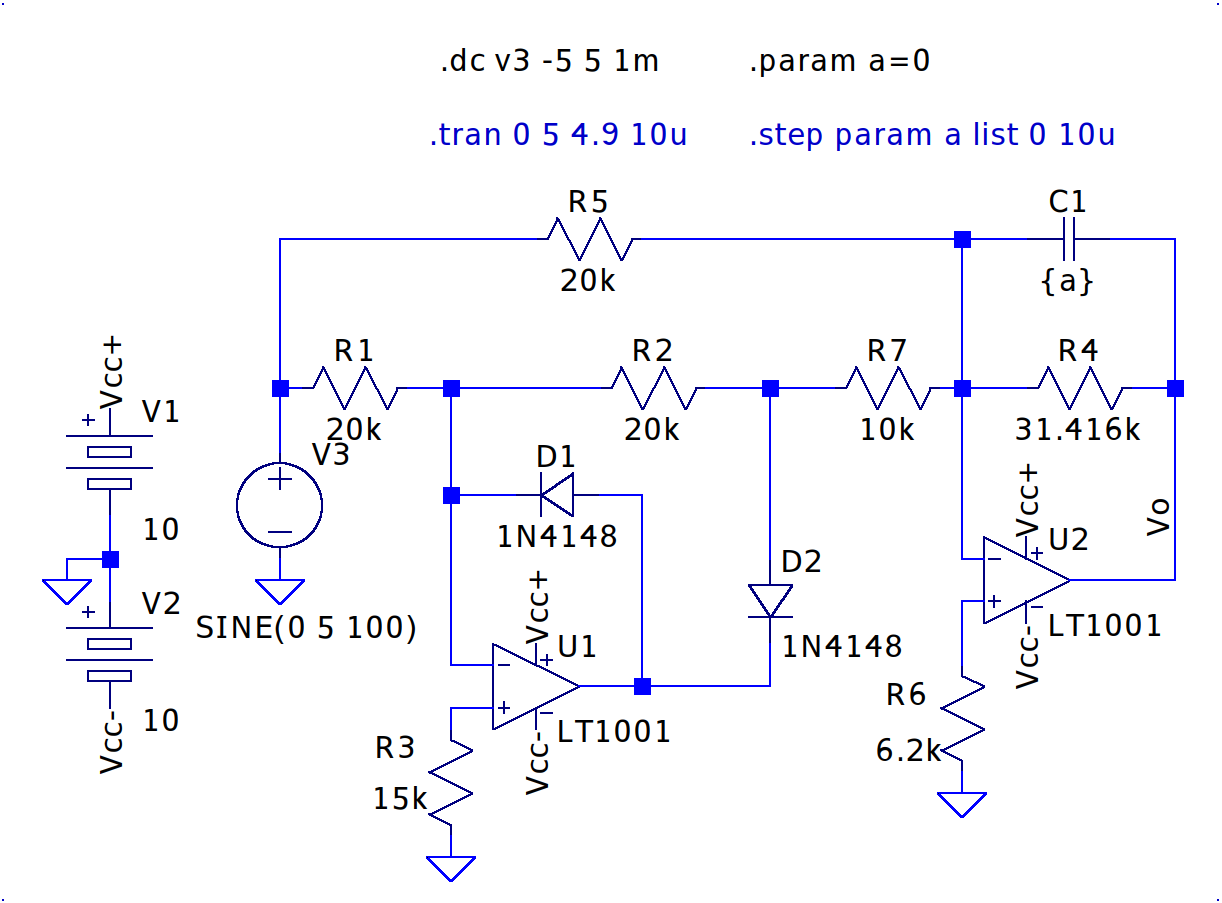
\includegraphics[width=0.8\linewidth]{figuras/oper20.png}
  	\caption{Circuito rectificador de onda completa para $C_1=0$ y conversor AC-DC para $C_1$ actuando como capacitor de filtro.}
  	\label{oper20}
  \end{figure}
  
  \begin{figure}
  	\centering
  	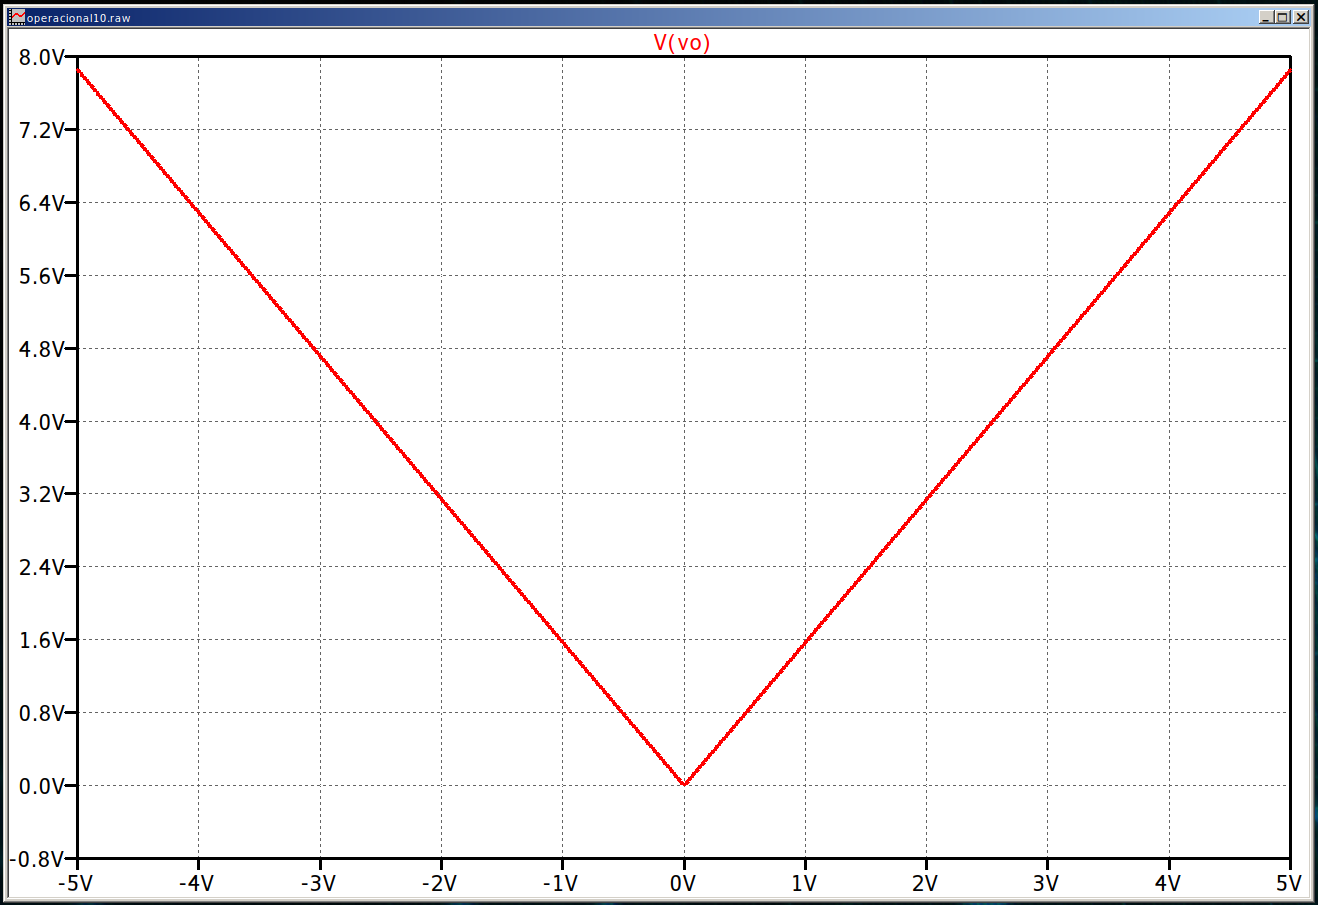
\includegraphics[width=0.8\linewidth]{figuras/oper21.png}
  	\caption{Transferencia del circuito de la figura \ref{oper20} con $C_1=0$.}
  	\label{oper21}
  \end{figure}
  
  
  \begin{figure}
  	\centering
  	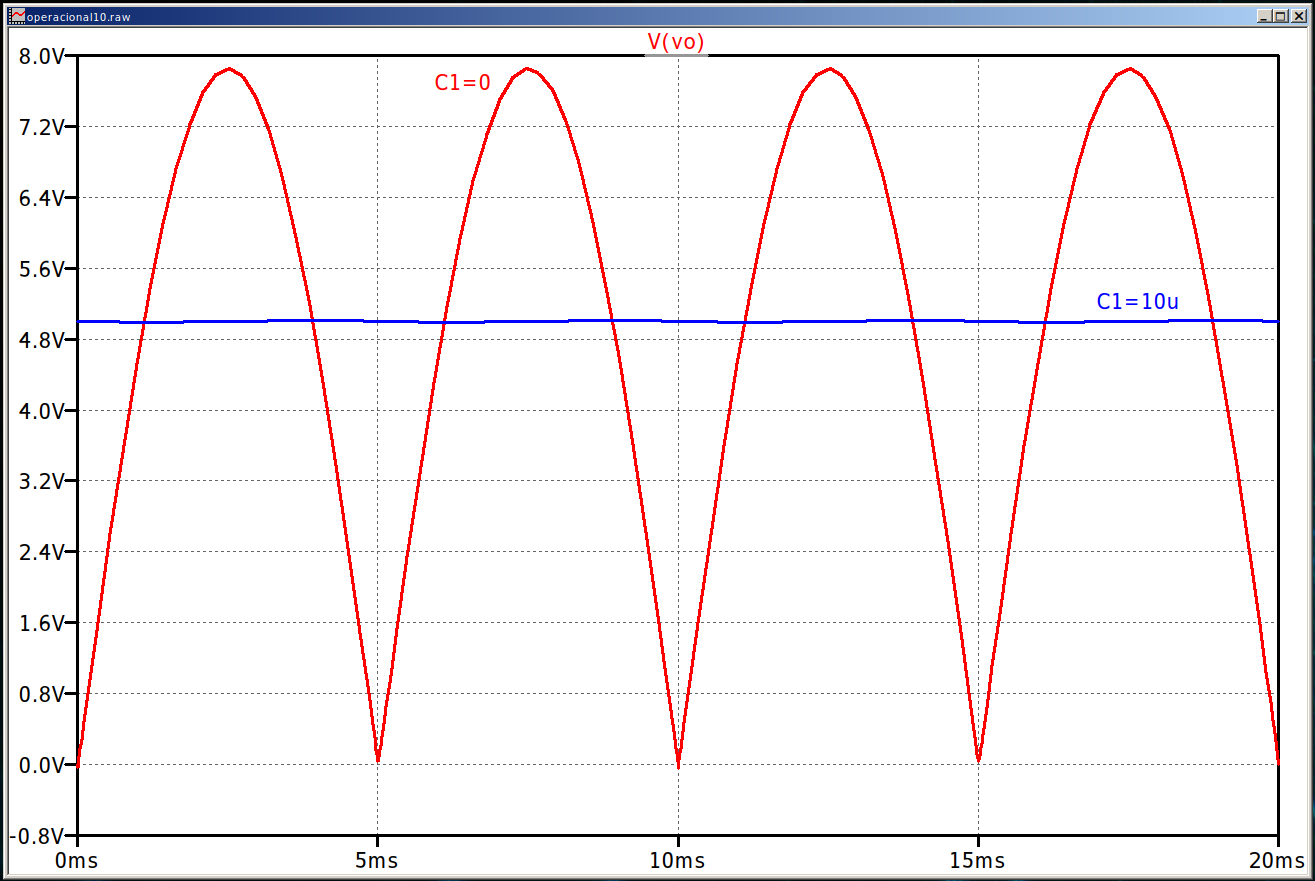
\includegraphics[width=0.8\linewidth]{figuras/oper22.png}
  	\caption{Respuesta temporal del circuito de la figura \ref{oper20} para $C_1=0$ y $C_1=10\mu$.}
  	\label{oper22}
  \end{figure}
  
  Otro ejemplo de circuitos que combinan operacionales y otros dispositivos semiconductores es el mostrado en la figura \ref{oper23}. En dicho circuito la entrada es la fuente $v_3$ que debe tomar siempre valores positivos, bajo esta restricción y debido al operacional $U_1$ la corriente de colector del transistor $Q_1$ será $i_{C1}=\frac{v_3}{R_6}$. Debido al operacional $U_2$ y al diodo Zener la corriente de colector del transistor $Q_2$ será $i_{C2}=\frac{V_Z}{R_1}$. Del circuito se ve que la salida $v_o$ es la resta de las tensiones base emisor de ambos transistores, es decir $v_o=v_{BE1}-v_{BE2}$, y como del modelo de los transistores bipolares se tiene que la corriente de colector es $i_C=I_s e^{\frac{v_{BE}}{V_T}}$, siendo $V_T=\frac{kT}{q}$ la tensión térmica en semiconductores, se deduce que:
  
%   \begin{equation}\label{ecuop7}
%  	v_o=-V_T \frac{i_{C1}}{i_{C2}} = -V_T  \frac{v_3R_1}}{R_6V_Z}
%   \end{equation}

 \begin{equation}\label{ecuop8}
	v_o= -V_T ln \frac{i_{C1}}{i_{C2}}=-V_T ln \frac{v_3R_1}{R_6V_Z}
\end{equation}

Como la tensión de Zener es en este circuito $V_Z$ es del orden de $6.2V$ y $R_6=10K$, si se ajusta en forma teórica $R_1$ a $62K$  y suponiendo una temperatura ambiente de $25^{\circ} C$,  el valor de la salida será $V_o=-25.7mV ln \displaystyle \frac{v_3}{1V}$, es decir la salida responde al logaritmo de la entrada cambiado de signo. 

En la simulación se puede ajustar el valor de $R_1$ colocando una fuente $v_3=1V$ y barriendo el punto de operación \emph{.op} mediante la directiva \emph{.step param a Rmin Rmax 0.01}, en un gráfico se obtiene el valor de $v_o$ en función de la resistencia $R_1$, tomando el valor de simulación de la misma para el caso de $v_o$ más próximo a $0V$. Bajo estas consideraciones en el circuito de la figura \ref{oper23} $R_1$ se ajustó a $63065,6\Omega$. 

Para comprobar la transferencia logarítmica teórica se aplica la directiva \emph{.dc v3 0.2 10 1m} dando como resultado lo mostrado en la figura \ref{oper24}. En el gráfico inferior se dibuja la salida $v_o$ en función de la entrada $v_3$, en el cual se verifca el ajuste para  que $v_o\approx0V$ cuando $v_3=1V$. En el superior se vuelve a graficar $v_o$ superpuesta con la respuesta teórica $-25.7mV ln \displaystyle\frac{v_3}{1V}$ verificando un comportamiento muy similar al teórico.

  \begin{figure}
 	\centering
 	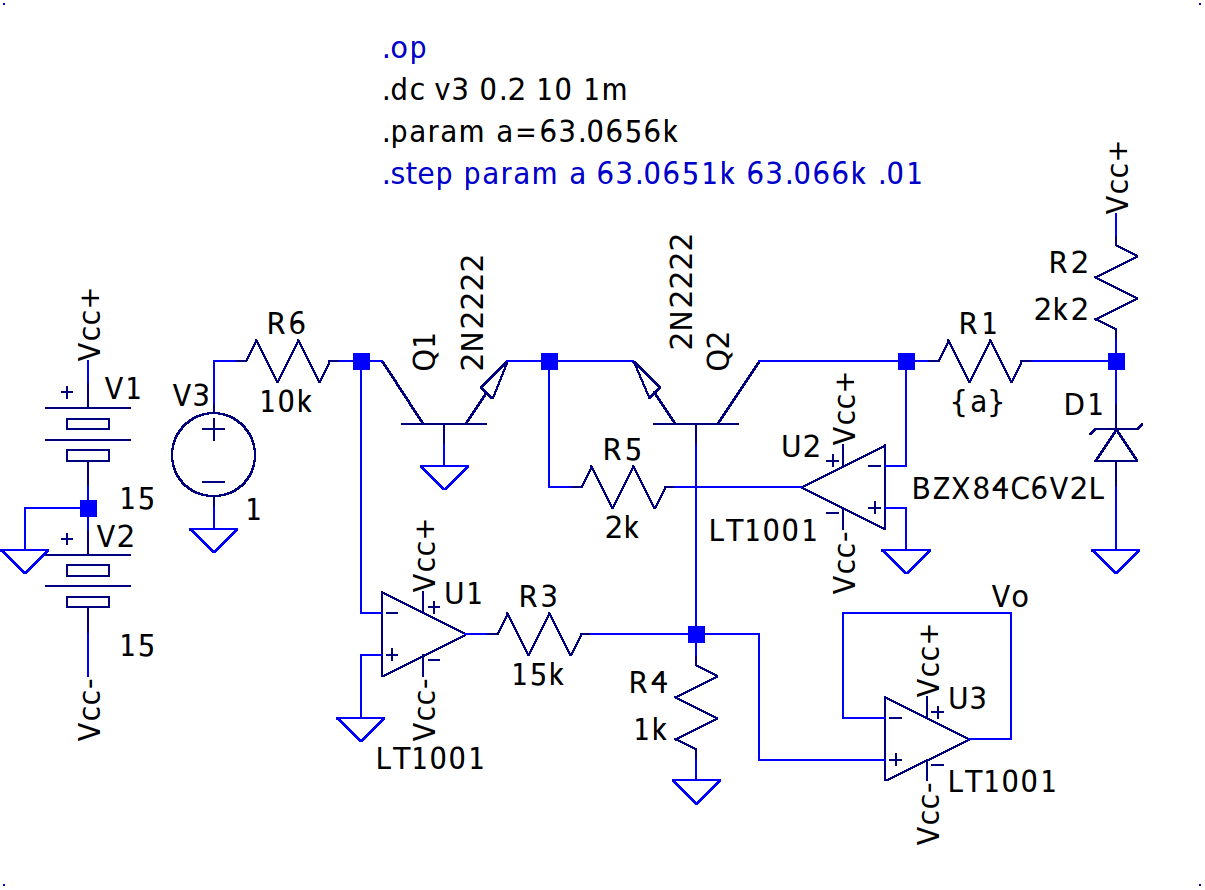
\includegraphics[width=0.8\linewidth]{figuras/oper23.png}
 	\caption{Circuito con transferencia logarítmica.}
 	\label{oper23}
 \end{figure}
 
 \begin{figure}
 	\centering
 	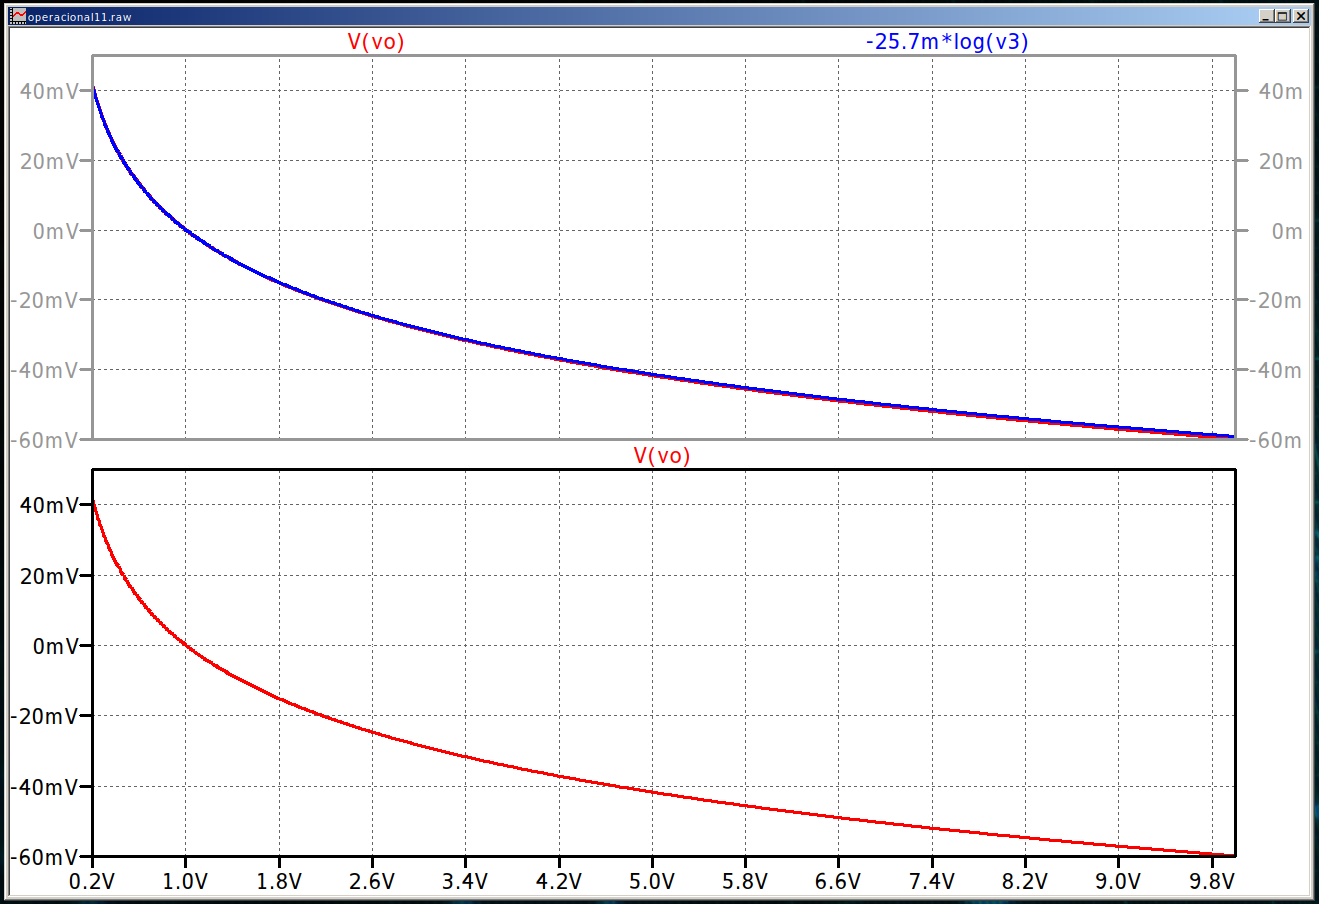
\includegraphics[width=0.8\linewidth]{figuras/oper24.png}
 	\caption{Simulación del circuito de la figura \ref{oper23}}
 	\label{oper24}
 \end{figure}




\section{Comparadores }
%
\hspace{10pt} Un amplificador operacional a lazo abierto o con realimentación positiva trabaja en forma no lineal, entregando una tensión de saturación a su salida con dos posibles valores: $V_o = \pm V_{sat} \approx \pm V_{cc}$, debido a que su gran ganancia de tensión hace que una muy pequeña diferencia de potencial en sus
entradas produzca saturación en la salida.

Los operacionales de propósitos generales pueden utilizarse como comparadores, aunque la compensación interna que poseen no los hacen óptimos para aplicaciones en las que se necesiten velocidades de respuesta elevadas. Para ello se utilizan circuitos integrados especialmente diseñados para trabajar como comparadores que tienen la ventaja de poder manejar entradas de tipo digital.

En la figura \ref{comparador1} se muestra un ejemplo de un circuito de comparación de tensión básico, a la izquierda se presenta un operacional a lazo abierto con una tensión de referencia de $2V$ en la entrada negativa y una señal senoidal $V_i$ de $8V$ de amplitud y $100Hz$ de frecuencia en la entrada positiva; a la derecha de la figura se muestra el mismo esquema circuital con una señal senoidal $V_r$  de $1V$ y $5KHZ$ superpuesta a $V_i$ emulando un posible ruido.

En la figura \ref{comparador2} se muestra la simulación temporal de ambos casos. El gráfico superior corresponde al circuito de la izquierda de la figura \ref{comparador1}, en él se ve que la salida $V_{o1}\approx +V_{cc}$ cuando la señal $V_i$ supera la tensión $V_{ref}=2V$ y $-V_{cc}$ en el caso contrario. En el gráfico inferior se muestra que el efecto del ruido superpuesto produce una incertidumbre en los momentos del cambio en la salida $V_{o2}$, pudiendo esta característica no ser aceptable en algunos diseños. 

  \begin{figure}
	\centering
	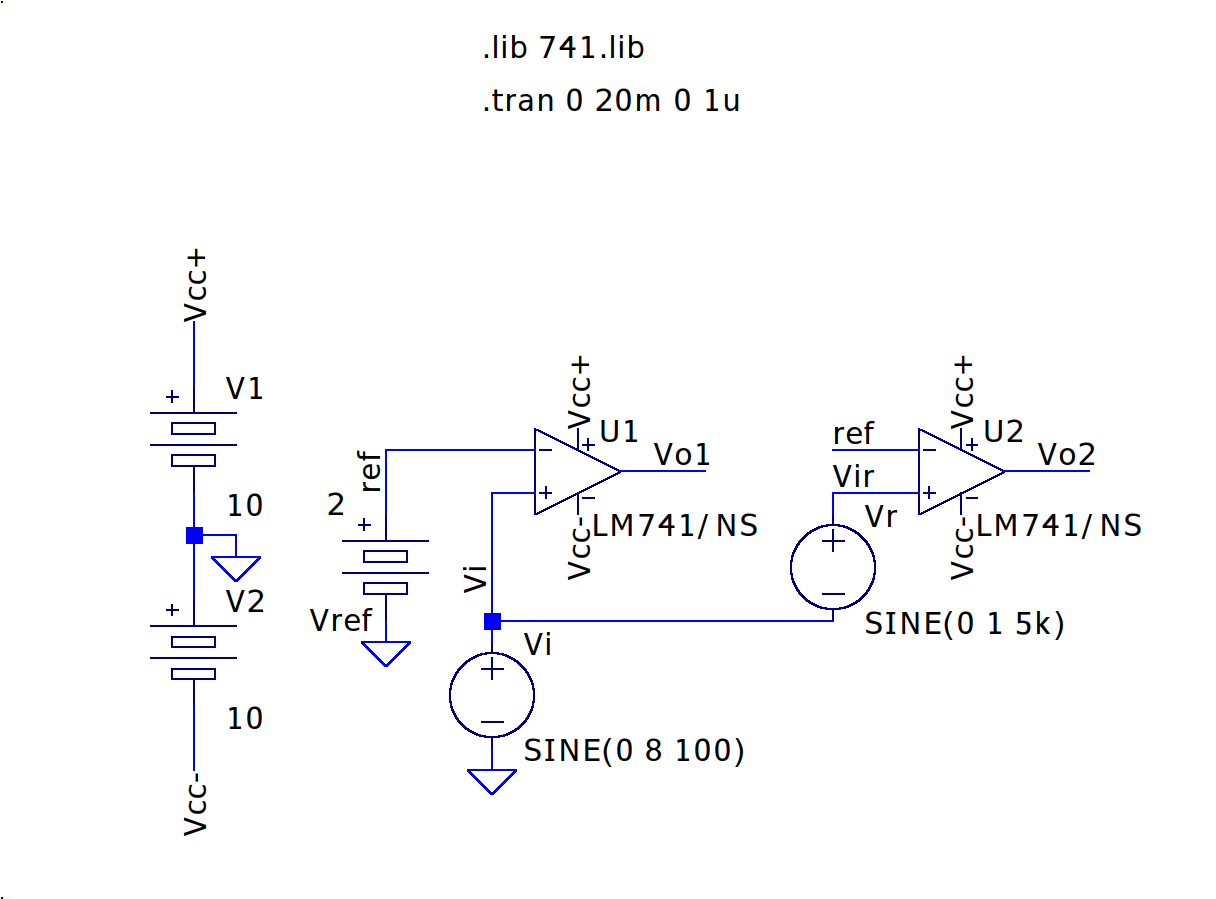
\includegraphics[width=0.8\linewidth]{figuras/comparador1.png}
	\caption{Comparador de tensión básico.}
	\label{comparador1}
\end{figure}

\begin{figure}
	\centering
	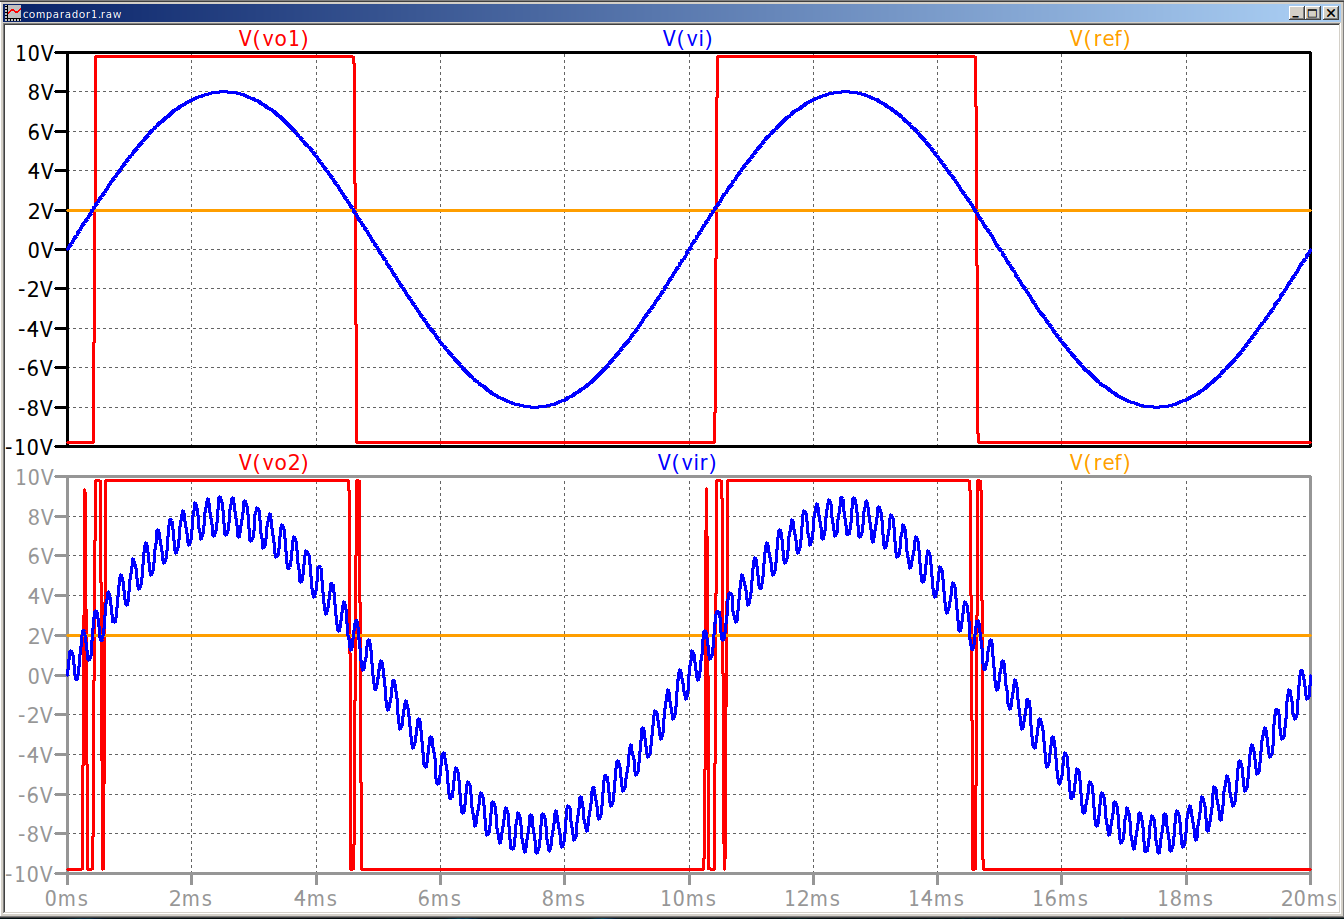
\includegraphics[width=0.8\linewidth]{figuras/comparador2.png}
	\caption{Simulación del circuito de la figura \ref{comparador1}}
	\label{comparador2}
\end{figure}

Para superar estos inconvenientes se diseñan comparadores con histéresis eléctrica que poseen niveles de comparación diferentes según el estado de la salida. El circuito de la figura \ref{comparador3} es un ejemplo  de este tipo de comparadores, dicho circuito presenta una realimentación positiva implementada con las resistencias $R_1$ y $R_2$, una tensión de referencia $V_{ref}$ conectada en la entrada inversora del operacional y la señal de entrada conectada a la red resistiva. Esta disposición circuital hace que la tensión en la entrada no inversora del operacional sea: 

 \begin{equation}\label{ecuop9}
	V^+=V_o \frac{R_1}{R_1+R_2} + V_i \frac{R_2}{R_1+R_2}  
\end{equation}

Considerando $R_2=nR_1$, que el operacional satura en $ \pm V_{cc}$ y que el punto para la modificación de la salida es cuando $V^+=V_{ref}$, se deduce que los valores de $V_i$ para el cambio de estado de la salida son:

  \begin{equation}\label{ecuop10}
  	\begin{split}
  		V_{i1}&=(n+1)V_{ref}-\frac{V_{cc}}{n}, \quad  Si \quad V_0=+V_{cc} \\
  		V_{i2}&=(n+1)V_{ref}+\frac{V_{cc}}{n}, \quad Si \quad V_0=-V_{cc}  
  	\end{split} 
  \end{equation}
  
  En la figura \ref{comparador4} se simula el circuito mencionado con una entrada $V_i$ que consiste en una rampa lenta que va de $-8V$ a $+8V$ en $1s$ y luego baja a $-8V$ en $1s$ (PWL(0-8 1 8 2 -8)). Se hace el análisis temporal que abarque $2s$ y se grafica la salida $V_o$ modificando el eje temporal por la señal de entrada $V_i$, obteniendo de este modo la transferencia del circuito visualizando que los niveles de comparación $V_{i1}$ y $V_{i2}$ cambian en función del valor de la salida.
  
  En la figura \ref{comparador5} se ve la simulación del circuito de la figura \ref{comparador3} cuando la entrada es una onda senoidal de $8V$ y $100Hz$ superpuesta con otra señal senoidal de $1V$ y $5KHz$ emulando ruido. Allí se verifica que la histéresis dada por $V_{i1}$ y $V_{i2}$ elimina la indeterminación en la comparación provocada por la señal de ruido  superpuesta.
  
  \begin{figure}
  	\centering
  	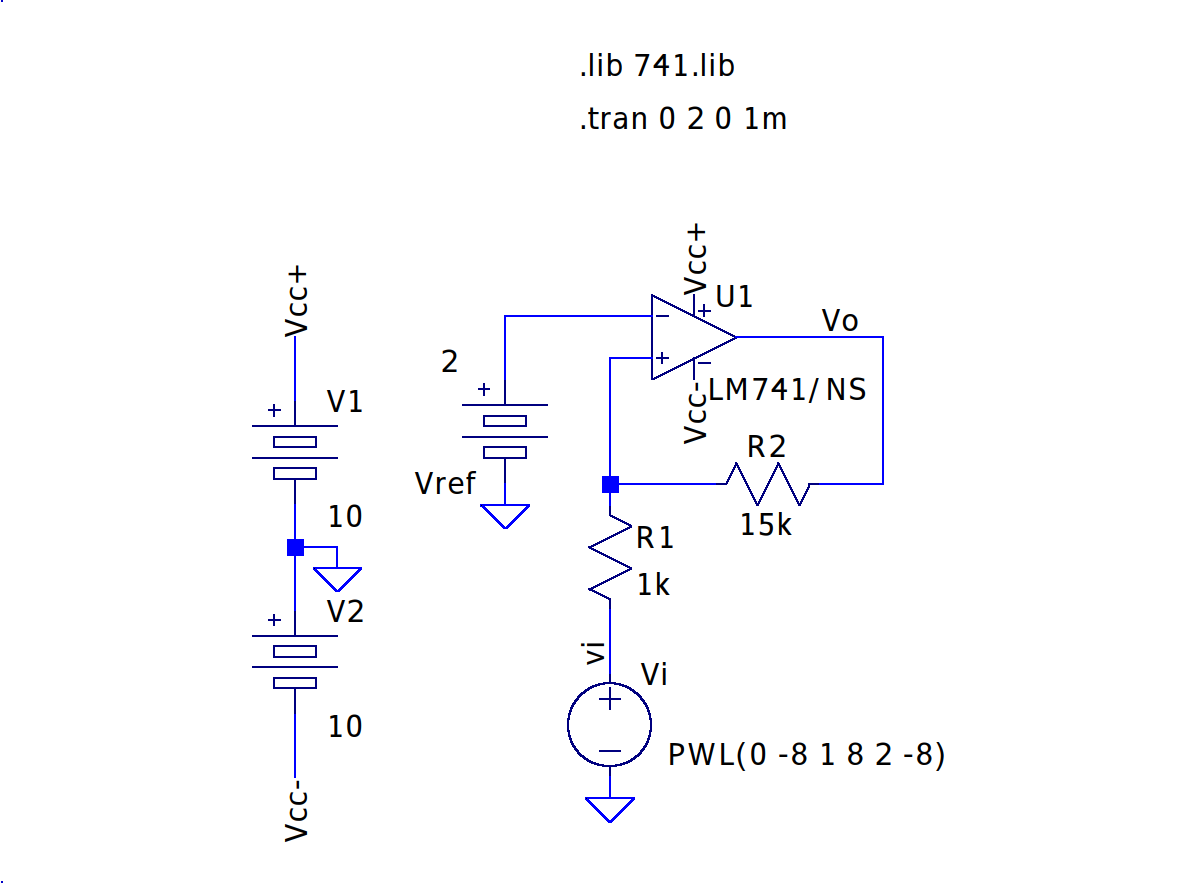
\includegraphics[width=0.8\linewidth]{figuras/comparador3.png}
  	\caption{Comparador de tensión con histéresis.}
  	\label{comparador3}
  \end{figure}
  
  \begin{figure}
  	\centering
  	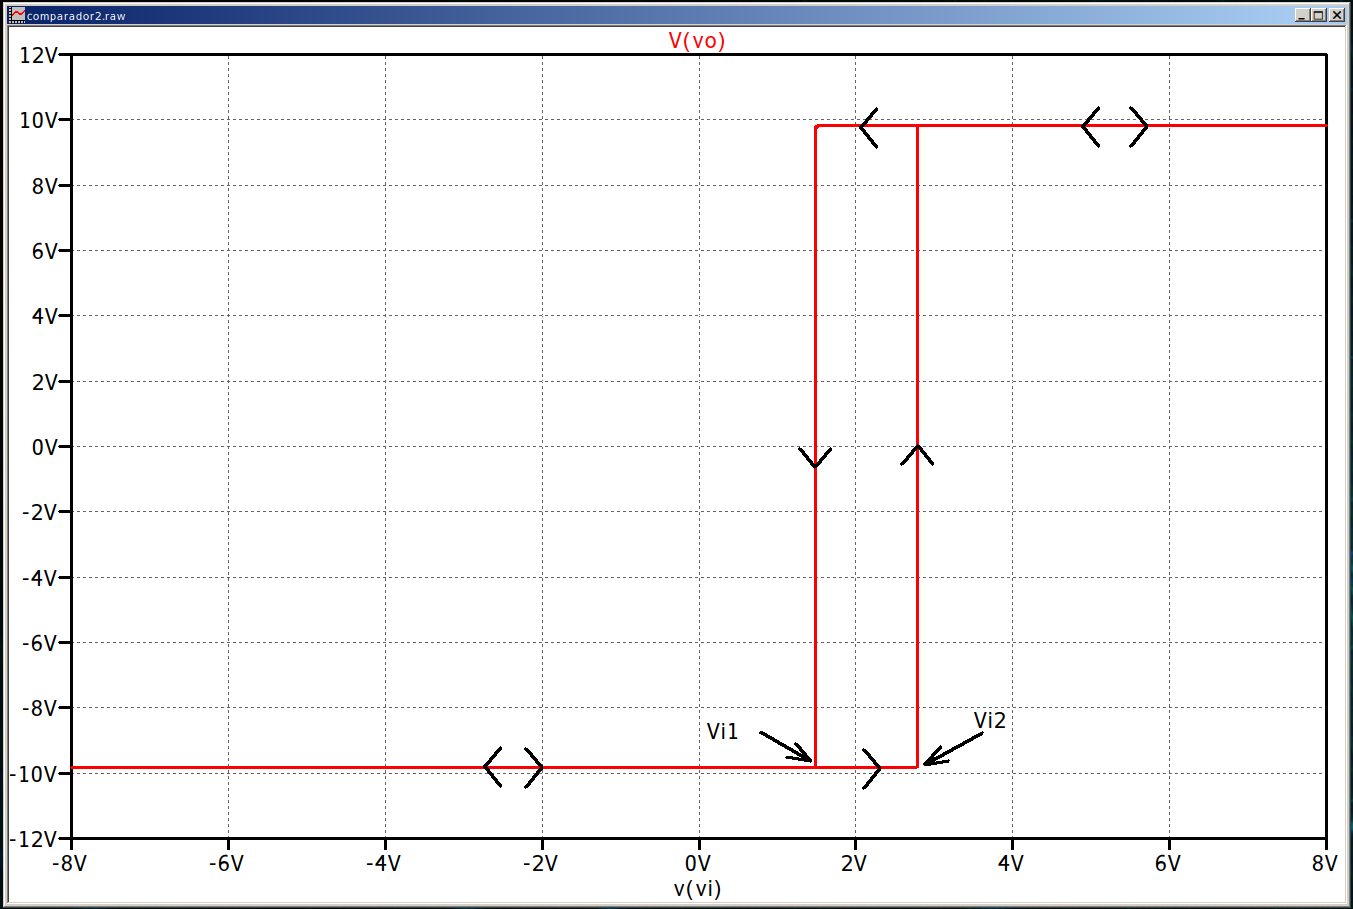
\includegraphics[width=0.8\linewidth]{figuras/comparador4.png}
  	\caption{Transferencia del circuito de la figura \ref{comparador3}}
  	\label{comparador4}
  \end{figure}
  
    \begin{figure}
  	\centering
  	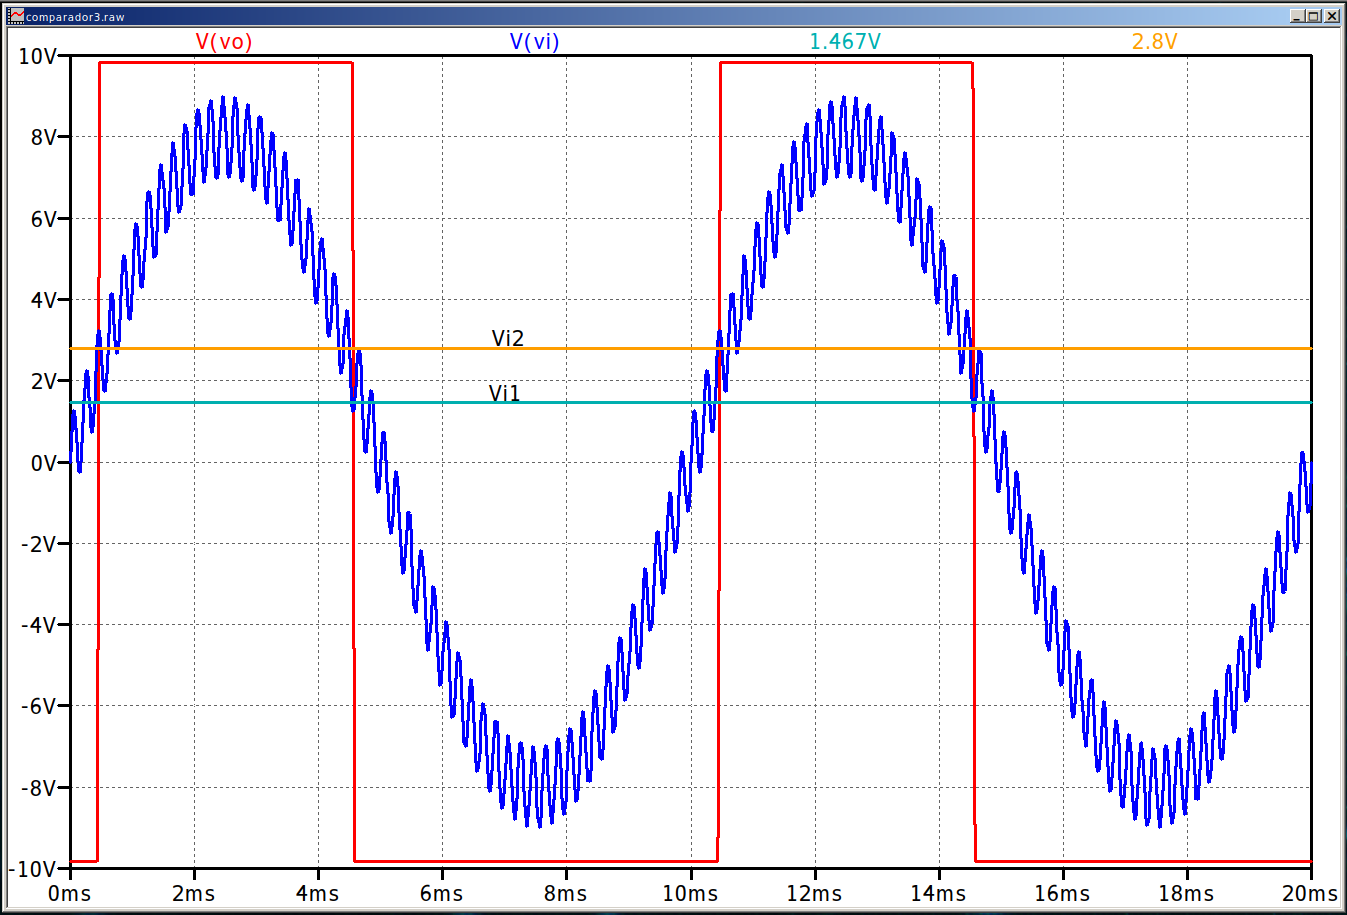
\includegraphics[width=0.8\linewidth]{figuras/comparador5.png}
  	\caption{Simulación temporal del circuito de la figura \ref{comparador3}}
  	\label{comparador5}
  \end{figure}
  
  Los comparadores se pueden utilizar también para generar señales periódicas en osciladores de relajación. La figura \ref{comparador6} es el esquema circuital de un generador de ondas triangular y cuadrada, el operacional de la izquierda actúa como comparador y el de la derecha trabajando en forma lineal dentro de un circuito integrador. En la figura \ref{comparador7} se muestran las formas de onda, cuadrada a la salida del comparador y triangular a la salida del integrador. Del análisis del circuito y considerando que $R_2=kR_3$, con $k\geq1$, y $\tau=R_1C_1$,  se desprende que la frecuencia teórica es
  $f_{o}=\frac{k}{4\tau}= 227.3Hz$ y la amplitud de la onda triangular es $V_p=\frac{V_{cc}}{k}=5V$. Por simulación, ver figura \ref{comparador7},  se obtuvo $f_o\approx 220.8Hz$ y $V_p\approx 4.99V$ que son valores crecanos a los predichos teóricamente.
  
  \begin{figure}
  	\centering
  	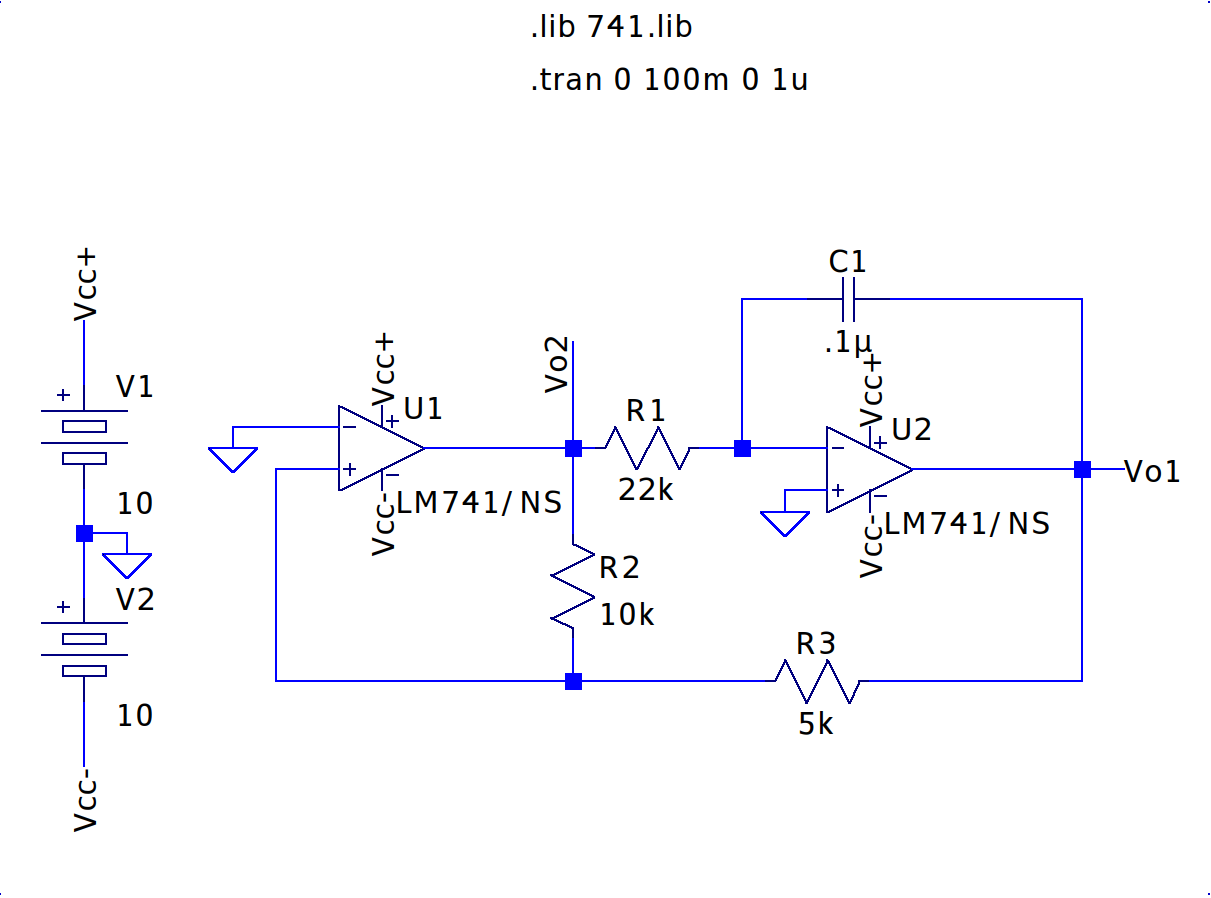
\includegraphics[width=0.8\linewidth]{figuras/comparador6.png}
  	\caption{Generador de señales cuadrada y triangular.}
  	\label{comparador6}
  \end{figure}
  
  \begin{figure}
  	\centering
  	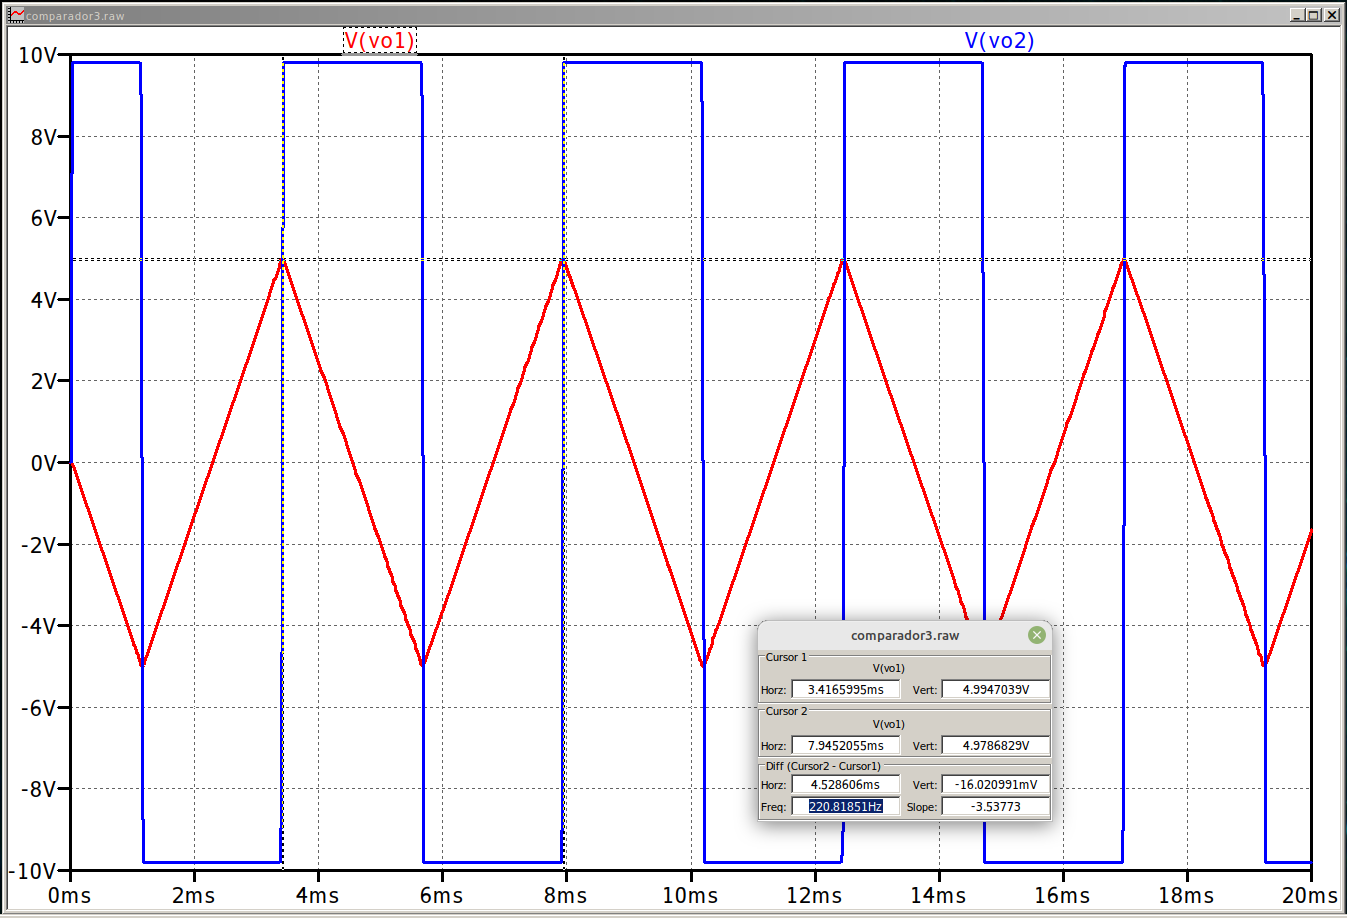
\includegraphics[width=0.8\linewidth]{figuras/comparador7.png}
  	\caption{Simulación temporal del circuito de la figura \ref{comparador6}}
  	\label{comparador7}
  \end{figure}